\documentclass[9pt]{sigplanconf}

\usepackage{amssymb}
\usepackage{amsmath}
\usepackage{amsthm}
\usepackage{stmaryrd}
\usepackage{color}
\usepackage{graphics}
\usepackage{fancyvrb}
\usepackage{subfigure}
\usepackage{amsthm}
\usepackage{tikz}
\usepackage{multirow}
\usepackage{minted}
\usepackage{breqn}

\fvset{
  linenos=true,
  fontsize=\footnotesize,
  breaklines=true,
  breakafter=+*,
  xleftmargin=\parindent
}

\usemintedstyle{vs}

\definecolor{darkblue}{rgb}{0.0,0.0,0.5}
\definecolor{darkgreen}{rgb}{0.0,0.4,0.0}
\definecolor{darkdarkgreen}{rgb}{0.0,0.35,0.0}

\usepackage[]{hyperref}
\hypersetup{
    unicode=false,          % non-Latin characters in Acrobat's bookmarks
    pdftoolbar=true,        % show Acrobat toolbar?
    pdfmenubar=true,        % show Acrobat menu?
    pdffitwindow=false,      % page fit to window when opened
    pdftitle={},    % title
    pdfauthor={}
    pdfsubject={},   % subject of the document
    pdfnewwindow=true,      % links in new window
    pdfkeywords={keywords}, % list of keywords
    colorlinks=true,       % false: boxed links; true: colored links
    linkcolor=darkblue,          % color of internal links
    citecolor=darkblue,        % color of links to bibliography
    filecolor=green,      % color of file links
    urlcolor=blue,          % color of external links
}


\CustomVerbatimEnvironment{SpecVerbatim}{Verbatim}{fontsize=\footnotesize,xleftmargin=0.5cm,
xrightmargin=0.2cm,commandchars=\\\{\},baselinestretch=0.98,numbersep=0.9em}
\CustomVerbatimEnvironment{ExmVerbatim}{Verbatim}{fontsize=\footnotesize,xleftmargin=0.5cm,
xrightmargin=0.2cm,baselinestretch=0.98,numbers=left,numbersep=0.9em,commandchars=\\\{\}}
\CustomVerbatimEnvironment{IVerbatim}{Verbatim}{fontsize=\relsize{-1},xleftmargin=0.5cm,
xrightmargin=0.2cm,commandchars=\\\{\},baselinestretch=0.98,numbersep=0.9em}


\definecolor{darkgreen}{rgb}{0.0,0.5,0.0}
\definecolor{darkpurple}{rgb}{0.6,0.0,0.6}
\definecolor{orange}{rgb}{0.8,0.4,0.0}
\definecolor{darkorange}{rgb}{0.5,0.2,0.0}
\definecolor{marco}{rgb}{0.0,0.3,0.5}
\definecolor{gray}{rgb}{0.2,0.2,0.2}

\newcommand\mdef{\stackrel{\mathclap{\normalfont\mbox{def}}}{=}}

\newcommand{\bn}{\mathbb{N}}

\newcommand{\dnote}[1]{\textcolor{darkpurple}{Dom: #1}}
\newcommand{\mnote}[1]{\textcolor{darkgreen}{Mistral: #1}}
\newcommand{\anote}[1]{\textcolor{red}{Andy: #1}}

\newcounter{block}

\newtheorem{lemma}[block]{Lemma}
\newtheorem{proposition}[block]{Proposition}
%\newtheorem{definition}[block]{Definisssstion}

\theoremstyle{definition}

\newtheorem{theorem}[block]{Theorem}
\newtheorem{remark}[block]{Remark}
\newtheorem{example}[block]{Example}
\newtheorem{definition}[block]{Definition}

% Writing macros
\newcommand{\ie}{\emph{i.e.}}
\newcommand{\eg}{\emph{e.g.}}

\newcommand{\dimId}{\texttt{dim}}

% Semantics related
\newcommand{\interp}[1]{\llbracket{#1}\rrbracket}

% Syntax macros
\newcommand{\nonterm}[1]{\textit{#1}}
\newcommand{\term}[1]{\texttt{#1}}

\newcommand{\stenRefl}[1]{\term{reflexive} \, (\term{dim=}#1)}
\newcommand{\stenFwd}[3]{\term{forward} \, (\term{depth=}#1,
  \term{dim=}#2{#3})}
\newcommand{\stenBwd}[3]{\term{backward} \, (\term{depth=}#1,
  \term{dim=}#2{#3})}
\newcommand{\stenCen}[3]{\term{centered} \, (\term{depth=}#1,
  \term{dim=}#2{#3})}
\newcommand{\irrefl}{\texttt{irreflexive}}

\newcommand{\stenReflS}[1]{\term{refl} \, (\term{dim=}#1)}
\newcommand{\stenFwdS}[2]{\term{fwd} \, (\term{depth=}#1,
  \term{dim=}#2)}
\newcommand{\stenBwdS}[2]{\term{bwd} \, (\term{depth=}#1,
  \term{dim=}#2)}
\newcommand{\stenCenS}[2]{\term{cen} \, (\term{depth=}#1,
  \term{dim=}#2)}
\newcommand{\irreflS}{\texttt{irrefl}}

\newcommand{\stenFwdSR}[3]{\term{fwd} (\term{depth=}#1,
  \term{dim=}#2, #3)}
\newcommand{\stenBwdSR}[3]{\term{bwd} (\term{depth=}#1,
  \term{dim=}#2, #3)}
\newcommand{\stenCenSR}[3]{\term{cen} (\term{depth=}#1,
  \term{dim=}#2, #3)}
\newcommand{\stenReflSR}[1]{\term{refl} (\term{dim=}#1)}

% SYNTAX OPERATIONS AND PREDICATES
\newcommand{\neigh}{\textsf{neigh}}
\newcommand{\arrayTy}{\textsf{array}}
\newcommand{\rhsExp}{\textsf{rhsExp}}
\newcommand{\var}{\textsf{var}}

%% VECTOR NOTATIONS
\newcommand{\vect}[1]{\textbf{#1}}
\newcommand{\vtwoh}[2]{\setlength{\arraycolsep}{0em}
\left[\begin{array}{cc}#1 \; & \; #2\end{array}\right]}
\newcommand{\vthreeh}[3]{\setlength{\arraycolsep}{0em}
\left[\begin{array}{ccc}#1 \; & \; #2 \; & \; #3\end{array}\right]}
\newcommand{\vtwo}[2]{\setlength{\arraycolsep}{0em}
\left[\begin{array}{l}#1\\#2\end{array}\right]}
\newcommand{\vthree}[3]{\setlength{\arraycolsep}{0em}
\left[\begin{array}{l}$#1$\\$#2$\\$#3$\end{array}\right]}
\newcommand{\stwo}[4]
%{\vtwo{#1}{#2}\!\vtwo{#3}{#4}}
{\setlength{\arraycolsep}{0.1em}
\left[\begin{array}{rr}$#1$ & $#3$\\$#2$ & $#4$\end{array}\right]}

\newcommand{\singleEntry}[2]{\textbf{J}_{#2}^{#1}}
\newcommand{\zeroEntry}[2]{\textbf{K}_{#2}^{#1}}

%% OPERATIONS ON SPANS and VECTORS
\newcommand{\containedin}{\sqsubseteq}

%% MODEL
\newcommand{\effdims}[2]{\mathit{constr}(#1)_{#2}}

\include{results}

\title{Verification of Stencil Computations through Spatial
  Specifications}
\authorinfo{Blind}{}{}
%\authorinfo{Dominic Orchard \and Mistral Contrastin
%\and Matthew Danish \and Andrew Rice}{University of Cambridge}{}

\begin{document}
\maketitle

\begin{abstract}
  Verifying the correctness of numerical computations relies on first
  giving a specification of their behaviour. In many cases, a
  numerical computation is derived from an underlying mathematical
  model, but this is often difficult to use as a specification as it
  is highly decoupled from the implementation. We have been studying
  specification techniques in middle ground between low-level and
  high-level specifications for numerical code. In this paper, we
  focus on \emph{stencil computations}---a common idiom in numerical code, but
  one which is error-prone due to fine-grained indexing errors. We
  hypothesise that in practise, stencil computations tend to have a
  regular shape which is amenable to static analysis and simple
  specification. We describe a abstract specification language for
  stencil computations that can be directly embedded as annotations in
  source code, along with an inference and checking procedure. We
  evaluate our language against a corpus of numerical Fortran code,
  and show that precise specifications can be given to roughly half of
  the identifiable stencil computations, and that the vast majority of
  stencil computations indeed have a simple, regular, static
  shape. This paper details our stencil specification language, its
  static semantics, inference, checking, and program synthesis
  procedures, our implementation, and our evaluation study. We provide
  an implementation of ontop of CamFort, an
  open-source program analysis and refactoring tool for Fortran corpus.
\end{abstract}

\keywords{program verification, specifications, static analysis,
  stencil computation}

\bibliographystyle{abbrvnat}

\section{Introduction}

\emph{Stencils} are a ubiquitous programming pattern, common in
scientific and numerical computing applications. Informally, a stencil
computation computes an array value, where the value at each index $i$ of
this array is calculated from a \emph{neighbourhood} of values around $i$ in
some input array(s), \eg{}, the Game of Life, convolutions in image
processing, approximations to differential equations. For example, the
following iteration computes the one-dimensional discrete Laplace
transform (an approximation to a derivative) in Fortran:
%
\begin{minted}{fortran}
do iter = 0, itermax
   do i = 1, (n-1)
      b(i) = a(i-1) - 2*a(i) + a(i+1)
   end do
   a = b
end do
\end{minted}
%
Line 3 is the core of the stencil computation, calculating
the value at \texttt{b(i)} from a neighbourhood of elements about
\texttt{a(i)}. Line 4 swaps
\texttt{a} and \texttt{b} between iterations, where \texttt{b} becomes the
input for the next iteration. In Fortran, parentheses \texttt{( )} are used
for array subscripts rather than the more familiar bracket syntax \texttt{[ ]}.

%This stencil computation exhibits statically decideable
%spatial and temporal relationships between $\texttt{a}$ and
%$\texttt{b}$.
In this simple example, the dependency between \texttt{a}
and \texttt{b} on line 3 forms a simple spatial relationship which is easily
understood. This spatial relationship determines other aspects of the
program and its efficient implementation: how much ``boundary'' is
needed for the array, the most cache-efficient layout in memory,
the partitioning shape for parallel implementations.

More complex stencil computations can be much harder to understand and
subsequently more prone to error. For example,
Figure~\ref{ref:navier-stokes-fragment} shows three lines from a
Navier-Stokes fluid simulator in which two arrays are read from with
different data access patterns, across two dimensions. The interaction
is much harder to understand, with the potential for the developer to
accidentally introduce an error via simple textual mistakes, for
example writing $\texttt{(i-1,j)}$ instead of $\texttt{(i+1,j)}$.

In this work, we introduce a simple specification language for the
spatial properties of stencil computations. The
specifications abstract over the fine grained detail of stencil access
patterns. In practice, most stencil computations have a regular shape
that can be described simply and abstractly, with a small set of
coarse-grained descriptions. In the case of our first Laplace example,
our inference procedure provides the specification:
%
\begin{minted}{fortran}
!=  stencil centered(depth=1, dim=1) :: a
\end{minted}
%
This explains that \texttt{a} is read from with a
symmetrical stencil pattern (``centered'') to a depth of one in each
direction in its first (and only) dimension.
%The second line explains
%the temporal relationship between \texttt{b} and \texttt{a}: that
%previous time step for \texttt{b} is actually provided by \texttt{a},
%and vice versa. This is explained as a mutual dependence between
%\texttt{a} and \texttt{b}.
In the case of the Navier-Stokes example of
Figure~\ref{ref:navier-stokes-fragment}, its inferred specification is shown
in Figure~\ref{ref:navier-stokes-fragment}(b). The
specification explains that, over the whole fragment, \texttt{u} is
read from with a centered pattern to depth of 1 in both dimensions
(this is known as the \emph{five point stencil}) and \texttt{v}
is read from in a neighbourhood bounded by forward to depth of $1$ in
the first dimension and backward to a depth of $1$ in the second
dimension. Figure~\ref{ref:navier-stokes-fragment}(c) describes these
pictorially.

In this paper, we make the following contributions:
%
\begin{itemize}
\item we introduce a specification language for
stencil computations that captures many common forms
of data access pattern, both spatial and temporal (Section~\ref{sec:lang});
\item we detail inference and checking
algorithms for stencil specifications (Section~\ref{sec:analysis});
\item we evaluate our implementation of the approach
in the CamFort tool for Fortran verification, studying
a number of example programs to assess the usefulness
of this approach.
\dnote{insert results here}
\end{itemize}
%

\begin{figure}[t]
\begin{minted}[firstnumber=20]{fortran}
du2dx = ((u(i,j)+u(i+1,j))*(u(i,j)+u(i+1,j))+ &
  gamma*abs(u(i,j)+u(i+1,j))*(u(i,j)-u(i+1,j))- &
  (u(i-1,j)+u(i,j))*(u(i-1,j)+u(i,j))- &
  gamma*abs(u(i-1,j)+u(i,j))*(u(i-1,j)-u(i,j))) &
  /(4.0*delx)

duvdy = ((v(i,j)+v(i+1,j))*(u(i,j)+u(i,j+1))+ &
  gamma*abs(v(i,j)+v(i+1,j))*(u(i,j)-u(i,j+1))- &
  (v(i,j-1)+v(i+1,j-1))*(u(i,j-1)+u(i,j))- &
  gamma*abs(v(i,j-1)+v(i+1,j-1))*(u(i,j-1)-u(i,j))) &
  /(4.0*dely)

laplu = (u(i+1,j)-2.0*u(i,j)+u(i-1,j))/delx/delx+ &
  (u(i,j+1)-2.0*u(i,j)+u(i,j-1))/dely/dely
\end{minted}
(a) Excerpt from Fortran code for a Navier-Stoke fluid simulator,
showing highly-detailed stencil computations. 
\vspace{0.5em}
\hrule
%
\begin{minted}{fortran}
!= stencil centered(depth=1,dim=1)*reflexive(dim=2) + centered(depth=1,dim=2)*reflexive(dim=1) :: u

!= stencil forward(depth=1,dim=1) * backward(depth=1,dim=2) :: v
\end{minted}
(b) Inferred stencil specification from CamFort.
\vspace{0.5em}
\hrule
%
\begin{center}
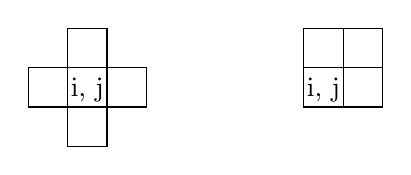
\begin{tikzpicture}
\node at (1.25,1.22) {i, j};
\draw (1,1) rectangle (1.5,1.5);
\draw (1.5,1) rectangle (2,1.5);
\draw (1,0.5) rectangle (1.5,1);
\draw (0.5,1) rectangle (1,1.5);
\draw (1,1.5) rectangle (1.5,2);
%
\node at (4.25,1.22) {i, j};
\draw (4,1) rectangle (4.5,1.5);
\draw (4.5,1) rectangle (5,1.5);
\draw (4.5,1.5) rectangle (5,2);
\draw (4,1.5) rectangle (4.5,2);
\end{tikzpicture}
\end{center}
\vspace{-0.3em}
(c) Pictorial representation of the two stencil specifications.
The horizontal dimension is \texttt{dim=1} and the vertical is \texttt{dim=2}.
\caption{Fragment of a Navier-Stokes fluid simulator and its
  specification in our language}
\label{ref:navier-stokes-fragment}
\end{figure}

\section{Stencil specification language}
\label{sec:lang}

Our specification system is based on the observation
that most forms of array access in numerical code have
a fixed, statically-determined access pattern. For example, the
``\emph{five-point stencil}'' on a two-dimensional array reads from array
indices $(i, j)$, $(i-1, j)$, $(i+1, j)$, $(i, j-1)$, and $(i, j+1)$
for all $i, j$ within the inner boundary of the array (to avoid
out-of-bounds access at the edges). We revisit this hypothesis
in Section~\ref{sec:evaluation} where the inference of
such regular stencil patterns on a corpus of numerical programs (both
small and large). We found that indeed \dnote{..}.

We outline the specification language here. Section~\ref{sec:syntax}
outlines the syntax. Section~\ref{sec:semantics} defines its semantics
via a simple set interpretation over indices. Section~\ref{sec:eqs} provides an
equational theory for specifications via relation ($\equiv$) and a
theory of approximation via relation ($<:$). These equations are then
proven sound with respect to the set semantics of Section~\ref{sec:semantics}.

\subsection{Notation and convention}
\label{sec:notation}

\renewcommand*{\arraystretch}{0.8}
\paragraph{Target language syntax} Throughout, for the source language
syntax, $v$ ranges over program variables, $s$ over statements, and
$e$ over expressions (which may be impure).  By ``variable'', we mean
in the imperative sense (\ie{}, named binders to memory cells) instead
of mathematical variables. We make clear a number of standard notions
used throughout.

\begin{definition}[Base induction variable]
  A variable \textit{v} of integer type is a \emph{base induction
    variable} if it is the control variable of a ``for''
  loop\footnote{Or equivalent for the target language, \eg{},
    \texttt{do} in Fortran for our implementation}, incremented by $1$ per
iteration. The variable is marked as a base induction variable
only within the scope of the loop, and such variables will be ranged
over by $i$, $j$, $k$. Since we do not use non-base induction
variables (which are traditionally affine transformations of induction
variables) we often simply say \emph{induction variable}.
\end{definition}

\begin{definition}[Array subscript]
  An \emph{array subscript} is an expression that indexes an array
  (for the purpose or reading or writing an element), which we denote
  by $v(\bar{e})$ for the source language where $\bar{e}$ is shorthand
  for a syntactic list of indexing expressions. A \emph{relative
    index} is a list $\bar{e}$ where each $e \in \bar{e}$ is defined
  in terms of some base induction variable.
\end{definition}

\begin{definition}[Neighbourhood index and neighbourhood subscripts]
  For an array subscript $v(\bar{e})$, we say that $e \in \bar{e}$
  is a \emph{neighbourhood index} if it is of the form
  $e \equiv i$, $e \equiv i + a$ or $e \equiv i - a$ where $a$ is a
  constant of integer type. That is, a neighbourhood index is a
  relative index defined as a constant translation of a base induction
  variable. The relation $\equiv$ identifies terms up-to commutativity
  of $+$ and the inverse relation of $+$ and $-$ (\eg{},
  $(-b) + i \equiv i - b$).  We classify neighbourhood indices using
  the predicate \neigh{}. An array subscript $v(\bar{e})$ where every
 $e \in \bar{e}$ is a neighbourhood index is called a
 \emph{neighbourhood subscript}.
\label{def:neighbour}
\end{definition}


\subsection{Specification syntax}
\label{sec:syntax}

Figure~\ref{fig:syntax} gives the syntax of stencil specifications,
which we introduces in stages below.  The top-level is given by the
\nonterm{specification} production which splits into either a
\nonterm{regionDec} (region declaration) or a \nonterm{specDec}
(specification declaration). Specification declarations associate a
specification to one or more program variables $\bar{v}$ (here given
using the Fortran style syntax of $\ldots \; \texttt{::} \bar{v}$),
describing how the array variables $\bar{v}$ are accessed.
%Specification declarations are either \nonterm{spatial} or
%\nonterm{temporal} specifications and describe, for spatial
%specifications,
%Specifications declarations describe
%how an array variable $v$ is read
%, and for temporal
%specifications what variables are used to define the array variable $v$.
%%

%\subsubsection{Spatial specification syntax}

\emph{Regions} are the central building blocks of spatial
specifications. Regions can either be declared along with a
\nonterm{regionDec}, assigning a region specification \nonterm{region} to
a region variable \nonterm{rvar} or given directly within a
\nonterm{spatial} specification.

\paragraph{Region constants}

Regions have as terminals the \emph{region constants}, denoted by
\term{reflexive}, \term{forward}, \term{backward}, or \term{centered}. Each
region constant except \term{reflexive} is given a depth parameter $n$ (natural
number greater than 0). They all receive a dimension identifier $d$ (also a
natural number greater than 0). Region constants specify that an array is read
from by a collection of indices which in the $d^{th}$ dimension are
neighbourhood indices ranging from $i + 0$ up to $i \pm n$ inclusively,
\eg{}, the following is valid stencil, reading from \term{a} and writing to
\term{b}:
%%
\begin{minted}{fortran}
!= stencil forward(depth=2, dim=1) :: a
b(i, 0) = a(i, 0) + a(i+1, 0) + a(i+2, 0)
\end{minted}
%%
were \texttt{i} is an induction variable.  The stencil specification
is associated to the array variable \texttt{a}. Note that the second
dimension is fixed at a constant here.

A \term{backward} stencil
is similar but has negative neighbourhood indices, \eg{},
%
\begin{minted}{fortran}
!= stencil backward(depth=2, dim=1) :: a
b(i) = a(i) + a(i-1) + a(i-2)
\end{minted}
%
A \texttt{centered} stencil is a combination of \texttt{forward}
and \texttt{backward} stencils to the same depth, \eg{},
%%
\begin{minted}{fortran}
!= stencil centered(depth=1, dim=1) :: a
b(i) = ( a(i) + a(i-1) + a(i+1) ) / 3.0
\end{minted}

\begin{figure}[t]
\begin{align*}
\def\arraystretch{1.2}
\setlength{\arraycolsep}{0.2em}
\newcommand{\dimTy}{\mathbb{D}}
\begin{array}{rl}
\nonterm{specification} ::= & \nonterm{regionDec} \mid \nonterm{specDec} \\
\nonterm{specDec} ::= & \term{stencil} \; \nonterm{spec} \;
                        \texttt{::} \; v
  \\
\nonterm{regionDec} ::= &  \texttt{region} \; \nonterm{rvar} \; \texttt{=} \;
                         \nonterm{region}\\[1em]
%\nonterm{spec} ::= & \nonterm{spatial} \mid \nonterm{temporal}
%\\[1em]
\nonterm{spec} ::= & [\nonterm{approx},] \; [\nonterm{mult},] \; \nonterm{region} \\
\nonterm{mult} ::= & \term{readOnce} \\
\nonterm{approx} ::= & \term{atMost} \; \mid \; \term{atLeast} \\[0.1em]
\nonterm{region} ::= & \\
\multicolumn{2}{l}{\qquad\qquad\;\;\; \stenFwd{\mathbb{N}_{>0}}{\dimTy}{\;[, \texttt{irreflexive}]}} \\
\multicolumn{2}{l}{\qquad\qquad \mid \; \stenBwd{\mathbb{N}_{>0}}{\dimTy}{\;[, \texttt{irreflexive}]}} \\
\multicolumn{2}{l}{\qquad\qquad \mid \; \stenCen{\mathbb{N}_{>0}}{\dimTy}{\;[, \texttt{irreflexive}]}} \\
\multicolumn{2}{l}{\qquad\qquad \mid \; \stenRefl{\dimTy}}  \\
\multicolumn{2}{l}{\qquad\qquad \mid \; \nonterm{region} \; \term{+} \; \nonterm{region}} \\
\multicolumn{2}{l}{\qquad\qquad \mid \; \nonterm{region} \; \term{*} \; \nonterm{region}} \\
\multicolumn{2}{l}{\qquad\qquad \mid \; \nonterm{rvar}}  \\[0.5em]
%\nonterm{temporal} ::= \; & \term{dependency} \; (v \; \{ , v \}) [, \texttt{mutual}]
%  \\[0.5em]
\dimTy ::= \; & \mathbb{N}_{>0} \\
\nonterm{rvar} ::= \; & [\text{\term{a}-\term{z}$\,$\term{A}-\term{Z}$\,$\term{0}-\term{9}}]+
\end{array}
\end{align*}
\caption{Specification syntax (EBNF grammar)}
\label{fig:syntax}
\end{figure}

\paragraph{Sum and product of regions}
%%
Region terms can be combined using the sum operator
\term{+} or the product operator \term{*}.

The sum of two regions $r \texttt{+} r'$ specifies that an array is
read using the neighbourhood indices described by either $r$ or
$r'$. It can be thought of as a disjunction of specifications. For
example, the following gives the specification for the five-point
stencil which is the sum of two compound \texttt{reflexive} and
\texttt{centered} regions in each dimension:
%%
\begin{minted}{fortran}
!= stencil centered(depth=1, dim=1)*reflexive(dim=2) + centered(depth=1, dim=2)*reflexive(dim=1) :: a

b(i,j) = -4*a(i,j) + a(i-1,j) + a(i+1,j)
                   + a(i,j-1) + a(i,j+1)
\end{minted}
%%
Here the left hand side of \texttt{+} says when the second dimension
(induction variable $j$) is fixed at the origin, the first dimension
(induction variable $i$) accesses immediate vicinity of the origin.
The right hand side of \texttt{+} is similar but the dimensions are reversed.
This reflects the symmetry under rotation in the fivepoint stencil.

The product of two regions $r \texttt{*} r'$ specifies that the array
is read with neighbourhood indices drawn from the bounding box created
by the regions two regions $r$ and $r'$. For example, the following
code (defining a nine-point stencil) has a specification as the
product of two \texttt{centered} regions in each dimension:
%%
\begin{minted}[breakindent=2.9em]{fortran}
x = a(i, j)   + a(i-1, j)   + a(i+1, j)
y = a(i, j-1) + a(i-1, j-1) + a(i+1, j-1)
z = a(i, j+1) + a(i-1, j+1) + a(i+1, j+1)

!= stencil centered(depth=1, dim=1) * centered(depth=1, dim=2) :: a
b(i, j) = (x + y + z) / 9.0
\end{minted}
%%
Such a stencil computation is a common image convolution (for example
for edge detection).
Note that there are a number of intermediate assignments over which
the whole specification ranges.

The region constructor \texttt{*} can also be interpreted as conjunction of
two specifications since they need to hold simultaneously for their
corresponding dimensions.

As another example, the following code and specification
implements the \emph{Roberts cross}
edge-detection convolution~\cite{davis1975survey}:
%%
\begin{minted}[breakindent=5.5em]{fortran}
do j=0, jmax-1
    do i=0, imax-1
      x = a(i,j) - a(i+1,j+1)
      y = a(i+1,j) - a(i,j+1)
      != stencil forward(depth=1,dim=1) * forward(depth=1,dim=2) :: a
      b(i,j) = sqrt(x*x+y*y)
   end do
end do
\end{minted}

\paragraph{Region declarations and variables}

Region specifications can be assigned to region variables via
a region declaration, which can be used later to form a spatial
specification. For example, the specification from the previous
 example can be restated as:
%%
\begin{minted}{fortran}
!= region r1 = centered(depth=1, dim=1)
!= region r2 = centered(depth=1, dim=2)
!= region robertsCross = r1*r2
!= stencil robertsCross :: a
\end{minted}
This is especially useful for common stencils such as Robert's cross
as the region can be defined once and used by region name many times.
%%
\paragraph{Spatial modifiers}
%%
There are two modifiers one used at specification the other at region
level to provide better descriptions for stencil computations.

At the specification level, the \texttt{readOnce} modifier enforces that no
index appears more than once. For example, in all of the previous examples the
\texttt{readOnce} modifier could be added, \eg{}
%
\begin{minted}{fortran}
!= stencil readOnce, backward(depth=2, dim=1) :: a
b(i+1) = a(i) + a(i-1) + a(i-2)
\end{minted}
%
However, this would be an invalid specification if any of the
array subscripts was repeated. This modifier provides a way to
rule out any accidental repetition of array subscripts.
The notion corresponds to that of \emph{linearity} in type systems,
though we opt for the more informative and easily understood name
\texttt{readOnce}. This modifier is optional, so it need not
be present even if the stencil is linear.

At the region level, \texttt{irreflexive} modifier qualifies base
regions of \texttt{forward}, \texttt{backward}, and \texttt{centered}.
It indicates that in the dimension of the region there is no neighbour index
with $0$ offset, \eg{},
%
\begin{minted}{fortran}
!= stencil centered(depth=1, dim=1, irreflexive) :: a
b(i) = a(i+1) + a(i-1)
\end{minted}
%
or with just a \texttt{forward} region an example would be:
%
\begin{minted}{fortran}
!= stencil forward(depth=1, dim=1, irreflexive) :: a
b(i) = a(i+1)
\end{minted}

Naturally, \term{irreflexive} qualifier cannot be used on \term{reflexive}
regions.

\paragraph{Under and over-approximation}

In some cases, it is useful to give a lower and/or upper bound for a
stencil. This can be done using either the \term{atMost} or
\term{atLeast} modifiers. This is particularly useful in situations
where there is a non-contiguous stencil, which does not fit the rest
of the specification syntax. For example:
%%
\begin{minted}{fortran}
!= stencil atLeast, reflexive(dim=1)      :: a
!= stencil atMost, forward(depth=2, dim=1) :: a
b(i) = a(i) + a(i+2)
\end{minted}
%%
%\subsubsection{Temporal specifications}


\subsection{Note on the design}

The names ``forward'', ``backward'' and ``centered''
are inspired by standard terminology in numerical analysis
for the shape of discretisation schemes. For example,
the standard ``explicit method'' for approximation
PDEs is the \emph{Forward Time, Centered Space} (FTCS)
scheme~\cite{dawson1991finite}. For
the one-dimensional heat equations, an FTCS discretisation
provides approximation code with the following stencil~\cite{recktenwald2004finite}:
%%
\begin{minted}{fortran}
do i=2, n-1
  u(i) = r*v(i-1) + r2*v(i) + r*v(i+1)
end do
\end{minted}
%%
where \texttt{r} and \texttt{r2} are some constants.
A valid specification for this stencil is then:
%%
\begin{minted}{fortran}
!= stencil centered(depth=1, dim=1) :: v
\end{minted}
%%
Such a specification can be inferred, or can be inserted by a user
and checked against the code.

\subsection{Equational theory and approximations}
\label{sec:eqs}

\begin{figure}
\begin{align*}
\setlength{\arraycolsep}{0.05em}
\begin{array}{c}
\framebox{$\textit{region} \equiv \textit{region}'$} \\[1em]
\begin{array}{rll}
(\textsc{F\, \texttt{+} \,F}) \;\; &
\stenFwdSR{n \, \textsf{max} \, m}{d}{r \vee s} \\
 \equiv \; & \stenFwdSR{n}{d}{r} \; \texttt{+} \; \stenFwdSR{m}{d}{s} \\[1em]
%
%
(\textsc{B\, \texttt{+} \,B}) \;\; &
\stenBwdSR{n \, \textsf{max} \, m}{d}{r \vee s} \\
 \equiv \; & \stenBwdS{n}{d}{r} \; \texttt{+} \; \stenBwdSR{m}{d}{s} \\[1em]
%
%
(\textsc{C\, \texttt{+} \,C}) \;\; &
\stenCenSR{n \, \textsf{max} \, m}{d}{r \vee s} \\
\equiv \; & \stenCenSR{n}{d}{r} \; \texttt{+} \; \stenCenSR{m}{d}{s} \\[1em]
%
%
(\textsc{C\, \texttt{+} \,F}) \;\; & \stenCenSR{n}{d}{r \vee s} \\
\textit{$m \leq n$} \; \equiv \; & \stenCenSR{n}{d}{r} \; \texttt{+} \;
                      \stenFwdSR{m}{d}{s} \\[1em]
%
%
(\textsc{C\, \texttt{+} \,B}) \;\; &
\stenCenSR{n}{d}{r \vee s} \\
\textit{$m \leq n$} \; \equiv \; & \stenCenSR{n}{d}{r} \; \texttt{+} \;
                      \stenBwdSR{m}{d}{s} \\[1em]
%
%
(\textsc{B\, \texttt{+} \,F}) \;\; &
\stenCenSR{n}{d}{r \vee s} \\
\equiv \; & \stenFwdSR{n}{d}{r} \; \texttt{+} \; \stenBwdSR{n}{d}{s}
  \\[1em]
%
%
(\textsc{R\, \texttt{+} \,F}) \;\; &
\stenFwdS{n}{d} \\
\equiv \; & \stenReflSR{d} \; \texttt{+} \; \stenFwdSR{n}{d}{r} \\[1em]
%
%
(\textsc{R\, \texttt{+} \,B}) \;\; &
\stenBwdS{n}{d} \\
\equiv \; & \stenReflSR{d} \; \texttt{+} \; \stenBwdSR{n}{d}{r} \\[1em]
%
%
(\textsc{R\, \texttt{+} \,C}) \;\; &
\stenCenS{n}{d} \\
\equiv \; & \stenReflSR{d} \; \texttt{+} \; \stenCenSR{n}{d}{r} \\[1em]
%
%
(\textsc{irrefl}) \;\; & (R \, \term{*} \, S^\irreflS) \, \term{+} \,
                         (R^\irreflS \, \term{*} \, S) \;
\equiv \; R \, \term{*} \, S \\[0.5em]
%
%
(\texttt{+}\textsc{idem}) \;\; & S \; \texttt{+} \; S \; \equiv \; S \\[0.5em]
%
(\texttt{+}\textsc{comm}) \;\; & S \; \texttt{+} \; T \; \equiv \; T \;
                       \texttt{+} \; S \\[0.5em]
%
(\texttt{+}\textsc{assoc}) \;\; & R \; \texttt{+} \; (S \; \texttt{+} \; T) \; \equiv \; (R \;
                       \texttt{+} \; S) \; \texttt{+} \; T \\[0.5em]
(\texttt{*}\textsc{comm}) \;\; & S \; \texttt{*} \; T \; \equiv \; T \;
                       \texttt{*} \; S \\[0.5em]
%
(\texttt{*}\textsc{assoc}) \;\; & R \; \texttt{*} \; (S \; \texttt{*} \; T) \; \equiv \; (R \;
                       \texttt{*} \; S) \; \texttt{*} \; T \\[0.5em]
(\textsc{dist}) \;\; & R \; \texttt{*} \; (S \; \texttt{+} \; T) \; \equiv \; (R \;
                       \texttt{*} \; S) \; \texttt{+} \; (R
                       \; \texttt{*} \; T)
\end{array}
%
%\framebox{${\textit{specDec} :: \texttt{v}} \equiv
%{\textit{specDec'} :: \texttt{v}}$} \\[1em]
%\begin{array}{rl}
% MUTUAL
%(\textsc{mutual}) \; &
%\texttt{stencil} \; \texttt{dependency} (\texttt{v}), \texttt{mutual}
%  :: \texttt{w}
%\\
%\equiv \; & \texttt{stencil} \; \texttt{dependency} (\texttt{w}), \texttt{mutual} ::
%  \texttt{v} \\[0.5em]
%(\textsc{coalesce}) \; &
%\texttt{stencil} \; \texttt{dependency} (\bar{v})
%  :: \texttt{v} \\
%& ; \texttt{stencil} \; \texttt{dependency} (\bar{w})
%  :: \texttt{v}
%\\
%\equiv \; & \texttt{stencil} \; \texttt{dependency} (\bar{v}, \bar{w}) ::
%  \texttt{v} \\[0.5em]
%\end{array}
\end{array}
\end{align*}
\caption{Equations on specifications}
\label{fig:equations}
\end{figure}

Figure~\ref{fig:equations} lists the equational theory for
specifications which is defined by the binary relation $\equiv$
between region terms. Stencil declarations are considered
equal when they have the same modifiers and $\equiv$ equates
their regions, \ie{}:
\begin{align*}
& \textit{region} \equiv \textit{region'} \\
& \quad \Rightarrow \;\; \texttt{stencil} \; [\textit{approx},] \; [\textit{mult},] \;
\textit{region} \\[-0.4em]
& \quad\quad \;\; \equiv \;\texttt{stencil} \; [\textit{approx},] \;
            [\textit{mult},] \; \textit{region}'
\end{align*}
%
To save space in the equations of Figure~\ref{fig:equations}, we use abbreviations
\term{refl}, \term{fwd}, \term{bwd}, and \term{cen} for \term{reflexive},
\term{forward}, \term{backward}, and \term{centered} regions
respectively. Futhermore, the abbreviations include syntactic sugar
for quantifying over the abseence or presence of the \irrefl{}
attribute on region constants as a boolean. For example,
the syntactic sugar in our equations for \term{fwd} is defined:
%%
\begin{align*}
& \stenFwdSR{n}{d}{r}
\; := \; \\[-0.4em]
& \qquad \begin{cases}
\stenFwd{n}{d}{, \irrefl} & \textit{if} \;\, \neg \, r \\
\stenFwd{n}{d}{}  & \textit{if} \;\,  r
\end{cases} \\
\textit{or} \;\;
& \stenFwdS{n}{d} := \stenFwd{n}{d}{}
\end{align*}
%
and similarly for \term{bwd} and \term{cen}.
We also frequently abbreviate \irrefl{} to \irreflS{}.

The equations reveal a partial semantics for stencil
specifications, which we briefly summarise.

\paragraph{Overlapping regions with +}
The first nine
equations (with labels of the form $\ldots \texttt{+} \ldots$)
explain the notion of \emph{overlapping} regions with sum
\term{+}. Note that in the first six, $r$ and $s$ range
over booleans denoting the absence (true) or presence (false)
of \irrefl{} which are combined via disjunction. For example,
the rule $(\textsc{B} \, \term{+} \,
\textsc{F})$ explains that the addition of \term{backward}
and \term{forward} regions in the same dimension and the same
depth is equivalent to a \term{centered} region of that depth.
If the \term{forward} part is irrefleixve (\ie{}, $r =
\textit{false}$) but \term{backward} is not (\ie{}, $s =
\textit{true}$) then their addition is equal to a \term{centered}
region with no \irrefl{} modifier by the disjunction ($r \vee s =
\textit{true}$), \ie{}:
%%
\begin{align*}
& \stenCenS{n}{d}  \\[-0.2em]
\equiv \;\; & \stenFwdSR{n}{d}{\irreflS} \; \texttt{+} \; \stenBwdS{n}{d}
\end{align*}
%%
That is, the \term{fwd} region is irreflexive describing code which is missing
a zero-offset neighbourhood index (\eg{}, missing $\texttt{a(i)}$), but the addition of
the \term{bwd} has no irreflexive attribute and thus provides the
missing zero offset index.

The equation (\textsc{irrefl}) explains an annihilation of
\irrefl{} using a further syntactic sugar.
We write $R^{\irreflS}$ to denote a region constant with an
irreflexive attribute, \eg{},
%%
\begin{align*}
\stenFwdS{n}{d}^{\irreflS} \, := \,
\stenFwdSR{n}{d}{\irreflS}
\end{align*}
%%
Thus, (\textsc{irrefl}) explains the sum of a
product of two regions $R$ and $S$ with itself,
where in each component of the sum one of $R$
or $S$ has the irreflexive attribute. These cancel to give
just the specification $R \, \term{*} \, S$.


\paragraph{Interaction between \term{+} and \term{*}}

The last six equations (from (\textsc{\term{+}idem}) inclusive), explain
the algebraic behaviour of \term{+} and \term{*}.  Together, we see
that \term{+} is an associative, commutative, idempotent binary
operator that distributes with \term{*}, which is associative and
commutative. This distribution of \term{*} over \term{+} is key as it
is used internally to give a normal form for stencil specifications
akin to Disjunctive Normal Form (DNF) (where \term{+} is taken as
``disjunction'' and \term{*} as the ``conjunction''). We revisit this
normalisation in Section~\ref{sec:inf-step4}.



\begin{figure}[t]
\begin{align*}
\begin{array}{c}
\dfrac{}{S <: S}(\textsc{refl}) \qquad \dfrac{R <: S \quad S <: T}{R <:
  T}(\textsc{trans}) \\[1.5em]
\dfrac{}{\texttt{readOnce} \, S <: S}(\textsc{rep})
\\[1.5em]
\setlength{\arraycolsep}{0.1em}
\dfrac{\hspace{3em} m \leq n \hspace{3em}}
{\begin{array}{rl}
\stenFwdS{m}{d} & <: \stenFwdS{n}{d}
%& \;\, ds \subseteq es \wedge n \leq m
\\
\wedge \stenBwdS{m}{d} & <: \stenBwdS{n}{d}
%& \;\, ds \subseteq es \wedge n \leq m
\\
\wedge \; \stenCenS{m}{d} & <: \stenCenS{n}{d}
%& \;\, ds \subseteq es \wedge n \leq m
\\
\wedge \; \stenBwdS{m}{d} & <: \stenCenS{n}{d} \\
\wedge \; \stenFwdS{m}{d} & <: \stenCenS{n}{d} \\[1em]
\end{array}} \\[2.5em]
\hspace{-0.5em}
\dfrac{S_1 <: T_1 \quad S_2 <: T_2}
      {S_1 \, \texttt{+} \, S_2 <: T_1 \, \texttt{+} \, T_2}
(\textsc{cong}\texttt{+}) \;\;\;
\dfrac{S_1 <: T_1 \quad S_2 <: T_2}
      {S_1 \, \texttt{*} \, S_2 <: T_1 \, \texttt{*} \, T_2}
(\textsc{cong}\texttt{*})
\end{array}
\end{align*}
\caption{Inequations on regions}
\label{fig:inequations}
\end{figure}

\paragraph{Inequations: sub-specifications}

Figure~\ref{fig:inequations}\dnote{TODO: this might
need to include notions of consistency}

\section{Semantics of specifications; a model}
\label{sec:semantics}

\newcommand{\domainVal}{\mathbb{Z}_\infty}

We define a semantic model for our stencil specification language.
This model has a number of purposes: (1) it is used in the inference,
checking, and program synthesis algorithms (introduced in
Section~\ref{sec:analysis}); (2) gives a basis for the equational
theory and approximations of the previous section; and (3) can be used
to guide correct implementations. The model is a denotational
semantics, in terms of sets of vectors which we call \emph{index
  schemes}. We introduce first the notion of indexing schemes
and \emph{unification} which gives the domain of our model
and forms the basis of the rest of the algorithsm for our
specificaiton. We then define the denotational model

\subsection{Indexing schemes and unification}

\begin{definition}[Index scheme]
An \emph{index scheme} is a vector of size $n$ (an $n$-vector)
with values drawn from $\domainVal = \mathbb{Z} \cup \{\infty\}$. 
Values in $\mathbb{Z}$ represent offsets 
of a neighbourhood index (indexing
expressions of the form $i + a$ where $i$ is an induction variable
and $a$ is a constant offset, Definition~\ref{def:neighbour},
p.~\pageref{def:neighbour}). The additional value
$\infty$ represents any indexing behaviour--- it is a 
wildcard.
Throughout $u, v, w$ range over index schemes, and $u_i$ denotes
the $i^{th}$ element of $u$. 
\end{definition}

Indexing schemes give an abstract
representation of index expressions in the source language.
Our model represents the meaning of stencil specifications
as indexing schemes, which explain the range of possible
indexing behaviours allowed under the specification.
The relationship between indexing schemes and source language
terms is given precisely by the partial function, \textsf{schematic}, which
maps syntactic array index terms to indexing schemes. This
operation forms the basis of the analysis required for the inference
and the checking procedures in Section~\ref{sec:analysis}. 

\begin{definition}[Schematic]
The partial function $\textsf{schematic}$ maps 
source-language indexing terms $(e_1, \ldots, e_n)$
into $n$-dimensional indexing schemes 
($\in \domainVal^n$), defined:
%
\begin{align*}
\mathsf{schematic}(e_1, \ldots, e_n) & = 
[\downarrow\!e_1 \ldots \downarrow\!e_n ] 
\quad \textit{iff} \; \forall i . \downarrow\!e_i \neq \bot 
\end{align*}
%
The $\downarrow$ operator is a partial\footnote{We represent
  partiality explicitly in our types with the set $A + \bot$.} function 
 $\downarrow : \textit{expr} \rightarrow (\domainVal + \bot)$
which maps each individal indexing expression to a component of
the indexing scheme, defined: 
%%
\begin{align*}
\downarrow\!e
 & =  \begin{cases}
a & e \equiv i + a \; \wedge \; \mathsf{neigh}(i + a) \\
-a & e \equiv i - a \; \wedge \; \mathsf{neigh}(i - a) \\
\infty & \textit{$\mathsf{IV}(e) = \emptyset$} \\
\bot   & \textit{otherwise}
\end{cases}
\end{align*}
%%
where $\mathsf{IV}(e)$ is the set of free induction variables
appearing in an expression, and $\neigh{}$ classifies expressions which 
are constant offsets from an induction variable
(Defn.~\ref{def:neighbour}). In the third case, 
if the expression is not a neighbourhood index but is not
a relative index either (\ie{} is not defined in terms
of an induction variable) then it is mapped to $\infty$, otherwise
$\downarrow\!e$ is undefined. The $\mathsf{schematic}$ function
is undefined if $\downarrow$ of any of its components $e_i$ is
undefined. 

For example $\textsf{schematic}(i, j+1) = \vtwoh{0}{1}$ assuming
$i$ and $j$ are induction variables and $\textsf{schematic}(i-1, 2, j)
 = \vthreeh{-1}{\infty}{0}$. However, $\textsf{schematic}(i*2, j)$, for
 example, is
 undefined as its first index is a non-neighbour relative index, which 
 is outside the scope of our specification language.
\end{definition}

\begin{definition}[Unification]
Two schemes $u, v$ of dimensionality $n$
are said to be \emph{unifiable}, written
$u \sim_n v$, iff the following holds:
%%
\[
u \sim_n v \; \Leftrightarrow  \;
  \forall i\!\in\!\{ 1,.., n \} . \, (u_i = \infty
\, \vee \, v_i = \infty \, \vee \, u_i = v_i)
\]
%%
That is, two schemes are related by the binary relation
$\sim_n$ over $(\mathbb{Z}_{\infty})^n$ if in each dimension
either is $\infty$ or they are equal. 
Thus, the element $\infty$ represents the ``general acceptor''
 meaning it unifies with any index in the same dimension. 

The subscript on $\sim_n$ is sometimes dropped when the
intended dimensionality is clear or inconsequential.
\end{definition}
 
 
%Unification relation, $\sim$, establishes whether
%a particular relativised subscript, $u$, of a group of subscripts involved
%in a stencil computation conforms with a unifier, $v$, of the model for
%the stencil computation.

\begin{example}
Take three array indexing terms
$(i, j+1)$, $(1, j+1)$ and $(3, j)$.
As given by \textsf{schematic}, these have the 
corresponding schemes: $\vtwoh{0}{1}$, $\vtwoh{\infty}{1}$
and $\vtwoh{\infty}{0}$ respectively. The following
relationship of unification (or lack of) then holds between
them:
%%
\begin{equation*}
\vtwoh{\infty}{0} \; \not\sim_2 \; \vtwoh{0}{1} \; \sim_2 \;
\vtwoh{\infty}{1} \; \not\sim_2 \; \vtwoh{\infty}{0}
\end{equation*}
%%
The middle pair unifies as $0$ and $\infty$ unify, 
whereas the left and right pairs do not unify as
$0 \not\sim_1 1$. 
\end{example}

Our terminology of \emph{indexing schemes} and
\emph{unification} are by analogy
with the \emph{type schemes} and \emph{type unification} of
ML~\cite{milner1978theory}, though our notion is much more rigid.


\subsection{Denotational model}

The model is given by the interpretation function $\interp{-}_n$
(where $n$ is the maximum dimensionality of the specification being
modelled) mapping closed\footnote{That is, we assume that there are no
  occurences of \textit{rvar} in a specification being modelled.  Any
  \emph{open} specification containing region variables can be made
  closed by straightforward syntactic subtitution with a (closed) 
  \textit{region}.} specifications to sets of
$n$-dimensional indexing schemes. The interperation is overloaded on
\emph{regions} in Figure~\ref{fig:region-model} and on the top-level
of a specification \textit{spec} in Figure~\ref{fig:spatial-model}.

We first define some intermediate notations and definitions.

\begin{definition}A \emph{single-entry vector} of size $n$, denoted
$\singleEntry{r}{n}$, is a vector where the $r^{th}$ entry is $1$
and all others are $\infty$, \eg{}, $\singleEntry{1}{2} =
\vtwoh{1}{\infty}$ and $\singleEntry{2}{3} = \vthreeh{\infty}{1}{\infty}$.
Thus, a single-entry vector is an indexing scheme which unifies with
all other schemes which have $1$ as their $r^{th}$ entry,
describing a neighbour offset of $1$. 
%DAO don't understand this sentence:
%In particular the constrained
%requires a non-zero offset from the induction variable.
\end{definition}

\begin{definition}A \emph{zero-entry vector} of size $n$, denoted
$\zeroEntry{r}{n}$, is a vector where the $r^{th}$ entry is $0$ and all others
are $\infty$, \eg{}, $\zeroEntry{1}{2} = \vtwoh{0}{\infty}$.

Similarly to the single-entry vector, zero-entry vectors 
are also indexing schemes which unify with all other schemes
as long as the $r^{th}$ entry is $0$, representing indices at
the ``origin'' in dimension $r$. 
\end{definition}


\begin{figure}
\begin{align*}
%
% REGION model
%
\setlength{\arraycolsep}{0.2em}
\def\arraystretch{1.4}
\hspace{-0.2em}
\begin{array}{rl}
\multicolumn{2}{l}{\interp{\stenFwdSR{k}{d}{r}}_n\!=\!
 \{i\singleEntry{d}{n} \,|\, i \in \{1, ..., k\} \} \, \cup \, \{
                             \zeroEntry{d}{n} \mid r \}} \\
%%
\multicolumn{2}{l}{\interp{\stenBwdSR{k}{d}{r}}_n\!=\!\{i\singleEntry{d}{n} \,|\, i \in \{-k, ..., -1\} \}\!\cup\!\{
  \zeroEntry{d}{n} \,|\, r \}} \\
%%
\multicolumn{2}{l}{
\interp{\stenCenSR{k}{d}{r}}_n\!=\!\{i\singleEntry{d}{n} \,|\, i \in \{\text{-}k,..., k\}\!\setminus\!0 \}
\!\cup\!\{ \zeroEntry{d}{n} \,|\, r \}} \\
\interp{\stenReflS{d}}_n & = \{ \zeroEntry{d}{n} \} \\
%
% REGION PROD model
%
\interp{r_1 \; \texttt{$\ast$} \; r_2}_n &
= \interp{r_1}_n \otimes \interp{r_2}_n \\
%
%  REGION SUM model
%
\interp{r_1 \; \texttt{+} \; r_2}_n &
= \interp{r_1}_n \cup \interp{r_2}_n
\end{array}
\end{align*}\vspace{-0.75em}
%\textit{$a^m \in A$ means there are $n$ copies of $a$ in
%  the multi-set $A$}
\caption{Model of regions, $\interp{\textit{region}}$}
\label{fig:region-model}
\end{figure}

\noindent
The first four equations of Figure~\ref{fig:region-model}
give the meanings of the region constants as sets of indexing
schemes. The next two give the meaning of combining regions
by $\term{+}$ and $\term{*}$. 

\begin{example}
For a $2$-dimensional situation, 
\begin{align*}
& \interp{\stenCenS{2}{1}}_2 \\
= \; & \{i\singleEntry{1}{2} \,|\, i \in \{\text{-}2,..., 2\}\!\setminus\!0 \}
  \cup  \{ \zeroEntry{1}{2} \,|\, \textit{true} \} \\
= \; & \{-2\singleEntry{1}{2}, \, -\singleEntry{1}{2}, \,
  \singleEntry{1}{2}, \, 2\singleEntry{1}{2}\} \cup
  \{\zeroEntry{1}{2}\} \\
= \; & \{\vtwoh{-2}{\infty}, \vtwoh{-1}{\infty}, \vtwoh{0}{\infty}, 
\vtwoh{1}{\infty}, \vtwoh{2}{\infty}\} 
\end{align*}
Note the absboring behaviour of $\infty$ with respect to
multiplication. 
\end{example}
\noindent
The model of $\term{+}$ is the straightforward union of 
the models of subterms. The model of $\term{*}$ is
the tensor $\otimes$ of subterm models. The tensor 
is non-trivial; we give some informal intutition first.

\paragraph{$\otimes$ of models}

The intuition behind $\otimes$ is that it takes
all possible pairs of indexing schemes, treating them as the
lower and upper bounds of an $n$-dimensional rectangle from which the 
remaining vertices of the rectangle are generated (like a bounding
box). \eg{}:
%%
\begin{align*}
\{\vtwoh{1}{2}, \vtwoh{5}{6}\} \otimes \{\vtwoh{3}{4}\} = 
\{&\vtwoh{1}{2}, \vtwoh{3}{2}, \vtwoh{1}{4}, \vtwoh{3}{4}, \\
  & \vtwoh{3}{6}, \vtwoh{5}{4}, \vtwoh{5}{6}\}
\end{align*}
%%
Internally $\otimes$ takes a Cartesian product of the indexing
schemes (all pairs) and then combines each pair using the 
\emph{pairwise permutation} written $\bowtie$ (defined later)
which generates all possible interleavings of two vectors
(\ie{}, all possible non-deterministic choices between $u_i$ and
$v_i$ in each dimension). Some care is then taken over
how this interacts with $\infty$: pariwse permtuation
corresponds to non-determinstic choice, in each dimension $i$,
between two values $u_i$ and $v_i$, but if either 
is $\infty$ then the resultying pairwise permutation is 
filtered out if the dimension $i$ has \emph{any other scheme
in the model where $u_i \neq \infty$}, \eg{}:
\begin{align*}
\{\vtwoh{1}{\infty}\} \otimes \{\vtwoh{3}{4}\} = 
\{\vtwoh{1}{4}, \vtwoh{3}{4}\}
\end{align*}
% 
where $\vtwoh{1}{\infty}$ and $\vtwoh{3}{\infty}$ have been filtered.
With respect to the notion of unification, the 
%
%
% combines non-$\infty$ constraints
%of the unifiers in different dimensions into less accepting unifiers.
%This means an access pattern unifying with this unifier would require
%both models to be satisfied. Use of $dims$ gives the dimensions that
%constitutent models talk about and is used in the product to eliminate
%general unifier appearing in these dimensions. Allowing general unifier
%in these dimensions would prevent both models to be satisfied
%simultaneously.
%
The notion of which dimensioons $i$ have that \emph{any scheme in the model
has $u_i \neq \infty$} is represented by the \emph{constrained
dimensions} intermediate function:
%
\begin{definition}[Constrained dimensions]
Given an $n$-dimensional model $M$, the \emph{constrained dimensions}
of that model is a subset of $\{1, \ldots, n\}$ of 
the dimensions for which at least one scheme $u \in M$ has
a non-$\infty$ value in that dimension. That is:
%
\begin{align*}
\effdims{M}{n} =
\bigcup_{u \in M} \{i \mid i \in \{1,\ldots,n\} \, \wedge \, u_i \neq
  \infty\}
\end{align*}
For example, $\effdims{\{\vtwoh{0}{\infty},\vtwoh{\infty}{\infty}\}}{2}
 = \{1\}$.
\end{definition}

\begin{definition}The tensor $\otimes_n$ of $n$-dimensional
models is defined:
\begin{alignat*}{2}
& M \otimes_n N =
  \Bigg\{x \; \Bigg| \;
    \parbox{6cm}{$(u, v) \in M \times N $ \\[0.1em]
                 $\;\; \wedge \;\, j \in (\effdims{M}{n} \cup
                   \effdims{N}{n})$\\[0.1em]
                  $\;\; \wedge \;\, i \in \{1, \ldots, 2^n\} \, \wedge
                  \, x = (u \bowtie v)_i$ \\[0.1em]                   
                   $\;\; \wedge \;\, x_j \neq \infty$
                  } \Bigg\} 
\end{alignat*}
The first guard takes the Cartesian product of
the two models and quantifies over all pairings $(u, v)$. 
The second guard says that $j$ ranges of the constrained
dimensions for $M$ unioned with the constrained dimensions for $N$.
That is, every $j$ corresponds to a dimension in which 
either $M$ or $N$ has a scheme $u$ where $u_j \neq \infty$,
and thus is constrained. 

The $\bowtie$ \emph{pairwise permutation} 
constructs a $2^n \times n$ matrix ($2^n$-vector of
$n$-vectors), which is indexed by $i$ above
and then $j$. Using this, the $\otimes$ operation constructs the set
of schemes which are the 
pairwise permutations of every pair $(u, v)$ of schemes in the Cartesian
product of $M \times N$. These permuted schemes are only those
which have non-$\infty$ components in the constrained dimensions
given by each model, given by the guard $x_j \neq \infty$.

The pairwise permutation $u \bowtie v$ takes two vectors and builds the matrix
where the rows are all possible $n$-vectors generated by
non-deterministic picking each $i^{th}$ entry from either the
$i^{th}$ entry in $u$ or the $i^{th}$ entry in $j$. For example:
%
\begin{equation*}
\vthreeh{0}{1}{2} \bowtie \vthreeh{3}{4}{5} =
\left[
\setlength{\arraycolsep}{0.42em}
\begin{array}{cccccccc}
0 & 0 & 0 & 0 & 3 & 3 & 3 & 3 \\ 
1 & 1 & 4 & 4 & 1 & 1 & 4 & 4 \\
2 & 5 & 2 & 5 & 2 & 5 & 2 & 5
\end{array}
\right]
% \\
%\setlength{\arraycolsep}{0.5em}
%\left[\begin{array}{ccc}
%0 & 1 & 2 \\
%0 & 1 & 5 \\
%0 & 4 & 2 \\
%0 & 4 & 5 \\
%3 & 1 & 2 \\
%3 & 1 & 5 \\
%3 & 4 & 2 \\
%3 & 4 & 5
%\end{array}
%\right]
\end{equation*}
%
The $2^n$ unique choices for $\bowtie$ on $n$-vectors
corresponds to taking all bit-strings of length $n$ and
selecting from $u$ for $1$ and $v$ for $0$. Thus, we can
defined the pairwise permutation matrix as:
%
\begin{align*}
(u \bowtie v)_{i,j} & = b_{i,j} u_j + \neg b_{i,j} v_j
\end{align*}
%
where $b$ is a logical matrix where $b_{i,j}$ is the $j$-th bit of the integer
$i - 1$.
%%
\dnote{I didn't understand mistral's description of unification
wrt to $\tensor$. I can't work it out either! Mistral have another
go given my above explanation}
\end{definition}


%The main interpretation function is overloaded on lists of
%variable-spec pairs $\interp{\overline{v : S}}$,
%returning multisets of variable-relative-index pairs. This provides
%the top-level definition of the model, with $\interp{-}$ overloaded
%on $S$, $\interp{S}$ mapping to multisets of
%relative indices not associated to an array variable.


\begin{figure}
\begin{align*}
\setlength{\arraycolsep}{0.7em}
& \interp{\textit{approx}, \textit{mult}, \textit{region}}_n
= \interp{\textit{mult}}^m \; (\interp{\textit{approx}}^a \,
\interp{\textit{region}}_n)
\end{align*}
with interpretation on modifiers to $\textsf{Mult}$
and $\textsf{Approx}$ injections:
\begin{align*}
& \begin{array}{lll}
\interp{\varepsilon}^{a}   = \textsf{exact} &
\interp{\term{atMost}}^{a} \hspace{1.3em} = \textsf{upper} &
\interp{\term{atLeast}}^{a} = \textsf{lower} \\[0.3em]
\interp{\varepsilon}^{m} = \textsf{once}
& \interp{\term{readOnce}}^{m} = \textsf{mult} &
\end{array}\\[-1.5em]
\end{align*}
%

%\interp{approx\texttt{,} \; mult\texttt{,} \; region}_n = \\
%   \begin{cases}
%     \textsf{once}(\textsf{up}(\interp{\mathit{region}}_n)) &
%       \mathit{approx} = \texttt{atMost} \wedge \mathit{mult} = \texttt{readOnce} \\
%     \textsf{mult}(\textsf{up}(\interp{\mathit{region}}_n)) &
%       \mathit{approx} = \texttt{atMost} \wedge \mathit{mult} = \epsilon\\
%     \textsf{once}(\textsf{low}(\interp{\mathit{region}}_n)) &
%       \mathit{approx} = \texttt{atLeast} \wedge \mathit{mult} = \texttt{readOnce}\\
%     \textsf{mult}(\textsf{low}(\interp{\mathit{region}}_n)) &
%       \mathit{approx} = \texttt{atLeast} \wedge \mathit{mult} = \epsilon \\
%     \textsf{once}(\textsf{exact}(\interp{\mathit{region}}_n)) &
%       \mathit{approx} = \epsilon \wedge \mathit{mult} = \texttt{readOnce}\\
%     \textsf{mult}(\textsf{exact}(\interp{\mathit{region}}_n)) &
%       \mathit{approx} = \epsilon \wedge \mathit{mult} = \epsilon
%   \end{cases}
\caption{Model of specifications, $\interp{\textit{spec}}$}
\label{fig:spatial-model}
\end{figure}

\paragraph{Model of \textit{spec}}

\todo{Explain the injections and the domain here}

\subsection{Soundness}

Given the model defined in this section we can
consider soundness for the equational theory of
specifications and the notion of spatial approximation
on specifications. The proofs are given in our supplement.

\begin{theorem}[Soundness of equational theory]
\[
\overline{\texttt{v} : S}\equiv \overline{\texttt{u} : T}
\; \Rightarrow \;
\interp{\overline{\texttt{v} : S}} = \interp{\overline{\texttt{u} : T}}
\]
\end{theorem}

\begin{theorem}[Soundness of approximations]
\[
\overline{\texttt{v} : S} <: \overline{\texttt{u} : T}
\; \Rightarrow \;
\interp{\overline{\texttt{v} : S}} \subseteq \interp{\overline{\texttt{u} : T}}
\]
\end{theorem}

\section{Inference and checking}
\label{sec:analysis}

\noindent
We briefly sketch the algorithms for inferring and checking
specifications and for synthesising programs from specifications.
Checking and synthesis use the set-based semantic model of
Section~\ref{sec:semantics}.

\paragraph{Syntax functions}
The function \rhsExp{} maps statements to a
set of expressions which occur in right-hand positions (\ie{}, not the
target of an assignment). The function \var{} maps expressions to a
set of the variables used in right-hand positions.

\subsection{Inference\label{subsec:inference}}

We demonstrate the main steps of the inference procedure over the
following example program which computes the mean value
of a five-point stencil at each index of the input array:
%%
\begin{minted}{fortran}
do i = 1, (n-1)
   do j = 1, (m-1)
      x       = a(i-1, j) + a(i+1, j)
      y       = a(i, j-1) + a(i, j+1)
      b(i, j) = (a(i, j) + x + y) / 5.0
   end do
end do
\end{minted}
%%
\subsubsection{Step 1: Standard control and data-flow analyses}
\label{sec:inf-step1}

The inference relies on some standard program analyses, computed
before the main inference procedure:
%
\begin{enumerate}
\item basic blocks (CFG);
\item induction variables per basic block;
\item (interprocedural) data-flow analysis, providing a \emph{flows to}
  graph (as shorthand, the function
  $\mathsf{flowTo}$ is used, implicitly parameterised by this graph,
  mapping an expression to the set of all expressions
  with forwards data-flow to this expression, based on the transitive
  closure of the flows graph);
\item type information per variable, where we use the predicate
\arrayTy{} to classify variables of array type.
\end{enumerate}
%

\subsubsection{Step 2: Data-access analysis}
\label{sec:inf-step2}

For each assignment statement whose left-hand side is an array
subscript on neighbourhood indices, a finite map is computed which
maps array variables to a set of vectors representing array
subscripts.  This finite map contains all array subscript expressions
which flow to this statement. More formally, a function
$\textsf{analyse}$ is applied to each statement in a program with the
following clause:
%
\begin{align*}
\begin{array}{lr}
\textsf{analyse}(v(\overline{e_1}) = e_2)
 := \qquad\qquad & \textit{where} \; \neigh(\overline{e_1}) \wedge \arrayTy(v)  \\[0.3em]
\multicolumn{2}{l}{\qquad \bigcup\{v' \mapsto \{\textsf{schematic}(\bar{e})\} \mid v'(\bar{e}) \leftarrow \mathsf{flowsTo}(e_2),
  \arrayTy(v')\}}
\end{array}
\end{align*}
%
That is, we focus on assignments to an array subscript where each
indexing expression in $\bar{e}$ is a neighbourhood index.  For
all array subscripts that flow to the right-hand side of this
statement, a finite map is constructed, mapping each array variable
in this flow a set of indexing schemes for its subscripts, computed
with \textsf{schematic}.

For our example, the \textsf{analyse} function matches on
line 5, with the following set for $\textsf{flowsTo}(\texttt{a(i, j) + x +
  y})$:
%
\begin{align*}
\{\texttt{a(i-1, j)}, \texttt{a(i+1, j)}, \texttt{a(i, j-1)},
  \texttt{a(i, j+1)}, \texttt{a(i, j)}\}
\end{align*}
Subsequently the result of \textsf{analyse} on line 5 yields the map:
\begin{align*}
\texttt{a} \mapsto \{\vtwoh{-1}{0}, \vtwoh{1}{0},
          \vtwoh{0}{-1}, \vtwoh{0}{1}, \vtwoh{0}{0}\}
\end{align*}
%

\subsubsection{Step 3: Coalesce contiguous indices into regions}
\label{sec:inf-step3}

Let $M$ range over the finite maps generated by \textsf{analyse}.  For
each $v \in \mathsf{dom}(M)$, the algorithm then constructs a group
of regions (called \emph{spans}) which cover all contiguous groups of relative indices
(from $M(v)$) in the $n$-dimensional space.
Informally, indexing schemes are converted to pairs $u \mapsto (u,
u)$, defining the lower and upper bound of a unit span 
in $n$-dimensions. For
example, for the five point stencil there are five $1 \times 1$ spans.
%
\begin{center}
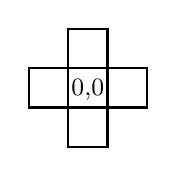
\begin{tikzpicture}
%\draw[step=0.5cm,lightgray,very thin] (0.5,0.5) grid (2,2);
\node at (1.25,1.22) {\textnormal{\small{0,0}}};
\draw[thick] (1,1) rectangle (1.5,1.5);
\draw[thick] (1.5,1) rectangle (2,1.5);
\draw[thick] (1,0.5) rectangle (1.5,1);
\draw[thick] (0.5,1) rectangle (1,1.5);
\draw[thick] (1,1.5) rectangle (1.5,2);
\end{tikzpicture}
\end{center}
%
Each dimension is traversed, coalescing consecutive spans
which vary in $m$-dimensions into coalesced spans which vary in
$m+1$-dimensions. In this example, the $0$-dimensional spans
 become $1$-dimensional spans (rows/columns):
%
\begin{align*}
\begin{array}{cc}
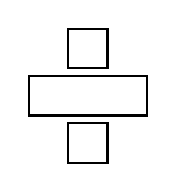
\begin{tikzpicture}
%\draw[step=0.5cm,lightgray,very thin] (0.5,0.5) grid (2,2);
%\node at (1.25,1.22) {\textnormal{\small{0,0}}};
\draw[thick] (0.5,1) rectangle (2,1.5);
\draw[thick] (1,0.40) rectangle (1.5,0.90);
\draw[thick] (1,1.60) rectangle (1.5,2.10);
\end{tikzpicture}
\qquad
&
\qquad
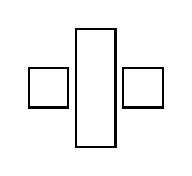
\begin{tikzpicture}
%\draw[step=0.5cm,lightgray,very thin] (0.5,0.5) grid (2,2);
%\node at (1.25,1.22) {\textnormal{\small{0,0}}};
\draw[thick] (1.6,1) rectangle (2.1,1.5);
\draw[thick] (0.4,1) rectangle (0.9,1.5);
\draw[thick] (1,0.5) rectangle (1.5,2);
\end{tikzpicture}
\\
\textit{dimension 1} \qquad & \qquad \textit{dimension 2}
\end{array}
\end{align*}
%
Any spans that are contained with any other span are deleted,
leaving a minimal set of spans (which may overlap, but none of which
fully contains another).
\begin{center}
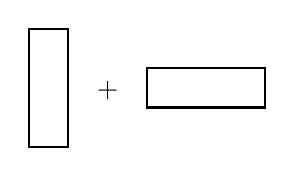
\begin{tikzpicture}
%\node at (1.25,1.22) {\textnormal{\small{0,0}}};
\draw[thick] (1,0.5) rectangle (1.5,2);
\node at (2,1.22) {+};
\draw[thick] (2.5,1) rectangle (4,1.5);
%\node at (2.75,1.22) {\textnormal{\small{0,0}}};
\end{tikzpicture}
\end{center}
%
This procedure is iterated till a fixed point is reached. In this
example this is reached in the first step. The final spans
are used to construct stencil specification, where
each span is product \texttt{*} of regions and multiple spans are
combined with the region sum \texttt{+}.

\newcommand{\spanOp}{\textsf{spans}}

Let $\vect{x}, \vect{y}, \vect{z}$ range over the column vectors of size
$n$ whose values are drawn from $\domainVal{}$.
We write $\vect{x}_{i:j}$ for the sub-vector from entry $i$ to
entry $j$ (inclusive).

\begin{definition}[Spans]
  A \emph{span} represents an $n$-dimensional box (\emph{hyper-rectangle}) as
  a pair of $n$-dimensional vectors (represented as a $2 \times n$
  matrix) giving the co-ordinates of the lower-bound vertex (first
  column) and the upper-bound vertex (second column). We use the
  notation $\vect{x} = [\vect{x}^L \; \vect{x}^U]$, where $\vect{x}^L$
  and $\vect{x}^U$ give the lower and upper bounds of the span.
\end{definition}

The algorithm to create contiguous spans, covering the space of
indices, then proceeds as follows.
Firstly, for all $v \in \mathsf{dom}(M)$ then a new map $M'$ is
created where each vector is mapped to the trivial \emph{unit span} is
created by pairing a vector with itself:
%
\begin{align*}
N(v) = \{[\vect{x} \;
  \vect{x}] \mid \vect{x} \in M(v)\}
\end{align*}
%
For our example, this yields:
%%
\begin{align*}
N(\texttt{a}) = \stwo{0}{0}{0}{0} \stwo{1}{0}{1}{0} \stwo{-1}{0}{-1}{0} \stwo{0}{1}{0}{1} \stwo{0}{-1}{0}{-1}
\end{align*}
%%
A fixed point is then compute for the following
procedure \spanOp which, for per variable
in the map, coalesces spans into contiguous regions in
the $n$-dimensional space. That is, we compute
 $(\mu \; \spanOp) N$ where \spanOp
is defined as follows for each variable in the map:
%
\begin{enumerate}

\item Compute all permutations on the column vectors in a span, \ie{},
  $[\vect{x}^L \vect{x}^U] \mapsto [\pi\vect{x}^L \, \pi\vect{x}^U]$
for a permutation $\pi$. For each permutation function $\pi^n_i$
(the $i$-th permutation for vectors of size $n$, we pair the
permutation function with the set of permuted spans so that
the spans can be un-permuted later.
%
\[
P(v) = \bigcup_{i \in n!} (\pi^n_{i} , \; \{[\pi^n_i
\vect{x}^L \; \pi^n_i\vect{x}^U] \, \mid \, [\vect{x}^L \; \vect{x}^U]
\leftarrow N(v)\}
\]
%
For our example, this yields:
%
\begin{align*}
P(\texttt{a}) =
\{&(\pi^2_1, \{ \stwo{0}{0}{0}{0},
\stwo{1}{0}{1}{0},
\stwo{-1}{0}{-1}{0},
\stwo{0}{1}{0}{1},
\stwo{0}{-1}{0}{-1} \})
\\
&(\pi^2_2, \{
 \stwo{0}{0}{0}{0},
 \stwo{0}{1}{0}{1},
 \stwo{0}{-1}{0}{-1},
 \stwo{1}{0}{1}{0},
 \stwo{-1}{0}{-1}{0}\})\}
\end{align*}
%
where $\pi^2_1$ is the identity permutation and $\pi^2_2$ is the
permutation flips the order of the two elements in the column
vectors.

\item Sort each permutation set into an ordered list, based on the ordering:
\begin{equation*}
  \vect{x} \leq \vect{y} =
      \exists i \, . \; \vect{x}_{i,1} \leq \vect{y}_{i,1} \; \wedge \;
        (i = n \vee \vect{x}_{i+1:n} = \vect{y}_{i+1:n})
\end{equation*}
%
This yields:
%%
\begin{align*}
\{&(\pi^2_1, [
\stwo{0}{-1}{0}{-1},
\stwo{-1}{0}{-1}{0},
\stwo{0}{0}{0}{0},
\stwo{1}{0}{1}{0},
\stwo{0}{1}{0}{1}] )
\\
&(\pi^2_2, [
\stwo{0}{-1}{0}{-1},
\stwo{-1}{0}{-1}{0},
\stwo{0}{0}{0}{0},
\stwo{1}{0}{1}{0},
\stwo{0}{1}{0}{1}])\}
\end{align*}
%%
\item Fold each list pairwise by the following partial operation
 $\bullet$ which coalesces contiguous regions:
%
\begin{align*}
& (\vect{x}^L,\vect{x}^U) \bullet (\vect{y}^L,\vect{y}^U) \\
= &
\begin{cases}
(\vect{x}^L, \vect{y}^U) & \vect{x}^U_1 + 1 = \vect{y}^L_1 \; \wedge \;
\vect{x}_{2:n} = \vect{y}_{2:n}) \\
\bot  & \textit{otherwise}
\end{cases}
\end{align*}
For our example, this yields:
%
\begin{align*}
Q(v) = \{&(\pi^2_1, [
\stwo{0}{-1}{0}{-1},
\stwo{-1}{0}{1}{0},
\stwo{0}{1}{0}{1}
]) \\
&(\pi^2_2, [
\stwo{0}{-1}{0}{-1},
\stwo{-1}{0}{1}{0},
\stwo{0}{1}{0}{1}])\}
\end{align*}
%
\item Un-permute and union together, \ie{},
%
\[
U(v) = \bigcup \{[\pi \vect{x}^L, \pi \vect{x}^U]
 \mid [\vect{x}^L, \vect{x}^U] \leftarrow S, (\pi, S) \leftarrow Q(v)\}
\]
Which yields:
%
\begin{align*}
U(\texttt{a}) =
\{\stwo{0}{-1}{0}{-1},
\stwo{-1}{0}{1}{0},
\stwo{0}{1}{0}{1},
\stwo{-1}{0}{-1}{0},
\stwo{0}{-1}{0}{1},
\stwo{1}{0}{1}{0}\}
\end{align*}
%
\item Finally, filter by the region containment predicate $\containedin$, that
  is, if any region is contained within another then remove the
  smaller. The $\containedin$ predicate is defined:
%
\begin{align*}
& (\vect{x}^L, \vect{x}^U) \containedin (\vect{y}^L, \vect{y}^U) = \\
& \vect{y}^L_1 \leq \vect{x}^L_1 \wedge \vect{x}^U_1 \leq \vect{y}^U_1
  \wedge (\vect{x}^L_{2:n}, \vect{x}^U_{2:n}) \containedin
  (\vect{y}^L_{2:n}, \vect{y}^U_{2:n})
\end{align*}
For our example this then yields the final result of:
\begin{align*}
\spanOp(M)
= \{\stwo{-1}{0}{1}{0} \stwo{0}{-1}{0}{1}\}
\end{align*}
since $\stwo{0}{1}{0}{1} \sqsubseteq \stwo{0}{-1}{0}{1}$
and $\stwo{1}{0}{1}{0} \sqsubseteq \stwo{-1}{0}{1}{0}$.
\end{enumerate}
For our example, applying \spanOp again yields the same
result, hence we have reached a fixed point.

\subsubsection{Step 4: Convert spans into specifications}
\label{sec:inf-step4}

\newcommand{\bplus}{\operatornamewithlimits{\term{+}}}
\newcommand{\tySum}[1]{#1^{\term{+}}}
\newcommand{\tyProd}[1]{#1^{\term{*}}}
\newcommand{\specDNF}{\textbf{spec}}
\newcommand{\result}[1]{\lfloor{#1}\rceil}

Next, the set of spans $\spanOp(M)$ covering the indexing
space is converted into abstract syntax trees 
for the specification language. This conversion is defined in terms
of an algebra on \textit{spec} syntax in disjunctive-normal form
(which we denote \specDNF{}). 

\begin{align*}
\result{\specDNF{}} = \specDNF + ((\specDNF{} + 1) \times
  (\specDNF{} + 1))
\end{align*}

\begin{align*}
\result{\specDNF{}} & ::= \textsf{exact} \, \specDNF{}
\mid \textsf{bounds} ([\specDNF{}], [\specDNF{}]) \\
\end{align*}

The algebra mirrors the shape
of the region combinators for addition and multiplication, 
with operators $\oplus$ and $\odot$ and a constructor for \specDNF{}:
%%
\begin{align*}
\oplus & : \specDNF \rightarrow \specDNF \rightarrow
  \specDNF \\
\odot & : \specDNF \rightarrow \specDNF \rightarrow
        \specDNF \\
\mathsf{toSpec} & : (\mathbb{Z} \cup \{\infty\}) \rightarrow (\mathbb{Z} \cup
  \{\infty\})  \rightarrow \specDNF
\end{align*}
%%
The $\mathsf{toSpec}$ operation takes a pair of lower and upper bounds
values (one-dimensional) and constructs a specification 
which contains a one-dimensional region. 
An entire span is converted into an $n$-dimensional
specification by applying $\mathsf{toSpec}$ to each
pair of lower and upper bounds in a span, per dimension, and multiplying these
specifications by $\odot$. The resulting specifications for
each span are then summed by by $\oplus$, that is, this step is given by:
\begin{equation*}
\textsf{spec}(M) = 
\sum\limits_{\vect{x} \in \spanOp(M)}
\prod\limits_{i \in \{1, \ldots, n\}} \, \mathsf{toSpec}(\vect{x}^L_i, \vect{x}^U_i)
\end{equation*}
(where $\oplus$ is the additive and $\odot$ is the multiplicative used
within $\Sigma$ and $\Pi$ respectively here).
We unpack the definitions of this algebra.

\begin{definition}[Specifications in DNF]
Let $r_1, ..., r_n$ range over elements of the \textit{region}
syntax (see Figure~\ref{fig:syntax}, p.~\pageref{fig:syntax}).
The set \specDNF{} is a subset of syntax trees \textit{spec}
of specifications in disjunctive normal form over regions 
where the disjunct is \term{+} (since its model is in terms of set
union) and the conjunct is \term{*} (since its model is a form of tensor).
That is elements of \specDNF{} are of the form:
%%
\[
(r^1_{1} \; \term{*} \ldots \term{*} \; r^1_n)\; \term{+} \; \ldots 
\term{+} \; (r^m_1 \, \term{*} \; \ldots \term{*} \; r^m_p)
\]
%%
More formally, $\specDNF \subseteq \textit{spec}$, defined:
%%
\begin{align*}
\specDNF{} & ::= [\textit{mult},] \;
\tySum{\specDNF} \\
\tySum{\specDNF} & ::= \tyProd{\specDNF} \; \term{+} \; \tySum{\specDNF} \mid
  \tyProd{\specDNF} \\
\tyProd{\specDNF} & ::= \textit{region} \; \term{*} \; \tyProd{\specDNF} \mid
   \textit{region}
\end{align*}
%%
In the following, $s, t$ range over elements of
\specDNF{}, $\tySum{s}, \tySum{t}$ range over elements of 
$\tySum{\specDNF}$ and $\tyProd{s}, \tyProd{t}$ range over elements
of $\tyProd{\specDNF}$ (for example, $\tyProd{s} = r^1_{1} \; \term{*}
\ldots \term{*} \; r^1_n$).
\end{definition}

\begin{definition} The $\mathsf{toSpec}$ constructor is defined:
%%
%\newcommand{\llower}{\vect{x}^L_i}
%\newcommand{\lupper}{\vect{x}^U_i}
\newcommand{\llower}{l}
\newcommand{\lupper}{u}
\begin{align*}
&\mathsf{toSpec} \; \llower \; \lupper = \\
&\begin{cases}
%% FWD
 \stenFwdS{\lupper}{i}  & \llower = 0 \, \wedge \, \lupper > 0 \\[0.2em]
 \stenFwdSR{\lupper}{i}{\irreflS}  & \llower = 1 \, \wedge \, \lupper > 0 \\[0.2em]
%% BWD
 \stenBwdS{|\llower|}{i}  & \llower < 0 \, \wedge \, \lupper = 0 \\[0.2em]
\stenBwdSR{|\llower|}{i}{\irreflS} & \llower < 0 \, \wedge \, \lupper = -1 \\[0.2em]
%% CEN
 \stenCenS{\lupper}{i}  & \llower < 0 \, \wedge \, \lupper > 0
 \, \wedge \, |\llower| = \lupper \\[0.2em]
 \stenBwdS{|\llower|}{i} & \llower < 0 \, \wedge \, \lupper > 0  \, \wedge \, |\llower| \neq \lupper \\
\quad \texttt{+} \, \stenFwdS{\lupper}{i}  & \qquad\quad \\[0.2em]
% BOUND
 \texttt{atMost}, \stenFwdS{\lupper}{i} & \llower > 1 \\[0.2em]
 \texttt{atMost}, \stenBwdS{|\llower|}{i} \quad & \llower < (-1)
 \\[0.2em]
% ABSOLUTE REP
 \epsilon & \llower = \infty \, \vee \, \lupper = \infty
  \end{cases}
\end{align*}
%%
The first two cases map to \texttt{forward} stencils since the lower
bound is $0$ or $1$, with the depth determined by the upper bound of
the span. If the lower bound is $1$, then the
$0$-offset point is missing so the region is given an
\texttt{irreflexive} attribute. The second two cases are similar for
\texttt{backward} but now the depth of the region is determined by the
absolute of the lower bound. In the fifth-case, where the lower bound
is negative and the upper bound is positive and they have the same
magnitude, then a \texttt{centered} region is constructed with
the depth as the common magnitude. If the magnitudes are not the same
(sixth case) then separated \texttt{forward} and \texttt{backward}
regions are summed, with their corresponding depths.

If the lower bound is greater than 1
(which implies the upper bound is greater than 1 too) then
this represents a region that is not at the origin (or next to) the
origin and thus cannot be represented in the specification language.
Thus, an upper bound is instead returned showing the maximum extent
of the region. The penultimate case is the dual, when the lower bound is less
than $-1$, giving an upper bound on a \texttt{backward} specification.

Finally, in the case where either bound is $\infty$, representing a non
neighbourhood index, then an empty specification is given
 with no regions, indicating that there is not even reflexive
0-offset access in this dimension.
\end{definition}

\begin{lemma}
$\mathsf{toSpec}$ is total (\ie{}, defined for all inputs)
 given the precondition that the lower
bound of the input span is less than or equal to its upper bound.
\end{lemma}

%\newcommand{\mkBig}[2]{\overset{\LARGE{\term{#1}}}{#2}}
\begin{definition} The $\odot$ operation on \specDNF{} is defined
\begin{align*}
& ([\textit{approx}_1] \; [\textit{mult}_1] \; 
\tySum{s})
\odot
([\textit{approx}_2] \; [\textit{mult}_2] \;
\tySum{t}) = \\
& \begin{cases}
\tySum{s} \tySum{\odot} \tySum{t} & \textit{approx}_1 =
\textit{approx_2} = \varepsilon
\\
\
& \textit{approx}_1 = \texttt{atLeast}, \textit{approx}_2 = \varepsilon
\end{cases}
\\
\end{align*}
\begin{align*}
s \tySum{\odot} t & =
 \bplus_{(\tyProd{s_1}, \tyProd{s_2}) \in (s \times
   t)} (\tyProd{s_1} \; \term{*} \; \tyProd{s_2})
%\begin{cases}%
%\end{cases}
\end{align*}
\end{definition}

\subsection{Checking\label{subsec:checking}}

Verification occurs when a user supplied specification is compared to the
actual access pattern. The mathematical model developed in
Section~\ref{sec:semantics} is used this comparison.

A specification is first synthesised into its model. Then access patterns
are checked against the model for consistency as defined in
Figure~\ref{fig:consistency}. The consistency predicate is defined recursively.
It first checks multiplicity if $\textsf{once}$ is at the top level, \ie{}
specification in question involves \texttt{readOnce} modifier, then array
accesses are checked for uniqueness using $unique$ predicate and the problem
is reduced to $\textsf{mult}$, which does not impose any extra constraints.
Next, consistency predicate considers whether the stencil is an approximation.
Semantically, a lower bound is achieved if every unifier in the model
correspond to some relativised vector of indices as that means all cells
described in the specification are part of the access pattern. Conversely,
an upper bound means all observed access patterns have a unifier. Hence,
the actual cells are a subset of the specified ones. In combination an
exact specification, \ie{} one without any approximation modifiers, is
one that is both a lower and an upper bound.

\begin{figure}
\begin{definition}
$unique(a,v)$ is the predicate indicating wheter indices vector of
array $v$ in assignment $a$ contain each element only once.
\end{definition}
\begin{dgroup*}
\begin{dmath*}
  \mathit{modelise}(a,v) =
  \begin{cases}
    \textsf{once}(\mathit{analyse}(a,v)) & unique(a,v) \\
    \textsf{mult}(\mathit{analyse}(a,v)) & otherwise
  \end{cases}
\end{dmath*}
\begin{dmath*}
  \mathit{check_n}(s,a,v) = \mathit{cons_n}(\interp{s}_n,\textsf{modelise}(a,v))
\end{dmath*}
\end{dgroup*}
%
\begin{dgroup*}
\begin{dmath*}
  \mathit{cons_n}(\textsf{once}(a),\textsf{once}(m)) =
    {\mathit{cons_n}(\textsf{mult}(a),\textsf{mult}(m)) }
\end{dmath*}
\begin{dmath*}
  \mathit{cons_n}(\textsf{mult}(\textsf{up}(m)),\textsf{mult}(m')) =
    {\forall u \in m' \; \exists v \in m \cdot u \preceq_n v }
\end{dmath*}
\begin{dmath*}
  \mathit{cons_}(\textsf{mult}(\textsf{low}(m)),\textsf{mult}(m')) =
    {\forall v \in m \; \exists u \in m' \cdot u \preceq_n v }
\end{dmath*}
\begin{dmath*}
  \mathit{cons_n}(\textsf{mult}(\textsf{exact}(m)),a) =
    {\mathit{cons_n}(\textsf{mult}(\textsf{low}(m)),a) \wedge
     \mathit{cons_n}(\textsf{mult}(\textsf{up}(m)),a) }
\end{dmath*}
\begin{dmath*}
  \mathit{cons_n}(\textsf{mult}(\textsf{both}(m_1,m_2)),a) =
    {\mathit{cons_n}(\textsf{mult}(\textsf{low}(m_1)),a) \wedge
     \mathit{cons_n}(\textsf{mult}(\textsf{up}(m_2)),a) }
\end{dmath*}
\end{dgroup*}

\caption{Consistency function of a model against stencil computation}
\label{fig:consistency}
\end{figure}

We will consider both a consistent and an inconsistent example to show how
checking works. The following is an example with a looser but still consistent
version of the \textit{fivepoint} stencil specification inferred previously in
the Subsection~\ref{subsec:inference}:
%
\begin{minted}[breakindent=8.1em]{fortran}
!= region fivepoint = centered(depth=1,dim=1) + centered(depth=1,dim=2)
!= stencil readOnce, fivepoint :: b
a(i,j) = b(i, j-1) + b(i,j) + b(i,j+1) + b(i-1,j) + b(i+1,j)
\end{minted}
%
\begin{enumerate}
\item Generate model from the specification as described in
  Section~\ref{sec:semantics}.
%
\begin{dmath*}
\interp{\texttt{stencil readOnce, fivepoint}}_2 =
  \textsf{once}(
    \textsf{exact}(
      \{ \vtwo{-1}{\infty},
          \vtwo{0}{\infty},
          \vtwo{1}{\infty},
          \vtwo{\infty}{-1},
          \vtwo{\infty}{0},
          \vtwo{\infty}{1}\}))
\end{dmath*}
%
\item Now $cons$ function is applied with this model along side with the
  assignment on line three and array $b$. For brevity the assignment is
  referred as $L3$ and the set of unifiers defined in the previous step as
  $m$.

  The predicate is reduced to
  $cons(\textsf{once}(\textsf{exact}(m)),L3,b)$.
%
\item $cons$ predicate from the previous step evaluates to
  $$unique(L3,b) \; \wedge \; cons(\textsf{mult}(\textsf{exact}(m)),L3,b).$$
%
  The former condition holds as no access pattern is repeated in $L3$ by simple
  inspection.
%
\item We further expand the function to 
  \begin{equation*}
    cons(\textsf{mult}(\textsf{up}(m)),L3,b) \wedge 
    cons(\textsf{mult}(\textsf{low}(m),L3,b).
  \end{equation*}
%
\item To evaluate the two predicates above, we need relativised indices for the
  array in question. This is obtained by $analyse$ function from
  Subsection~\ref{subsec:inference}.

  For the example above the relativised indices are as follows:
%
\begin{dmath*}
analyse(L3,b) =
  \{ \vtwo{0}{-1},
     \vtwo{0}{0},
     \vtwo{0}{1},
     \vtwo{-1}{0},
     \vtwo{1}{0}
  \}
\end{dmath*}
%
\item Below we present two match ups of relativised access patterns and unifiers
  to show both the lower and the upper bound holds.

  The unifications for the lower bound:
  \begin{align*}
     \vtwoh{0}{-1} & \sim_2 \vtwoh{0}{\infty} \\
     \vtwoh{0}{0} & \sim_2 \vtwoh{0}{\infty} \\
     \vtwoh{0}{1} & \sim_2 \vtwoh{0}{\infty} \\
     \vtwoh{-1}{0} & \sim_2 \vtwoh{\infty}{0} \\
     \vtwoh{1}{0} & \sim_2 \vtwoh{\infty}{0}
  \end{align*}

  The unifications for the upper bound:
  \begin{align*}
     \vtwoh{-1}{0} & \sim_2 \vtwoh{-1}{\infty} \\
     \vtwoh{0}{0} & \sim_2 \vtwoh{0}{\infty} \\
     \vtwoh{1}{0} & \sim_2 \vtwoh{1}{\infty}  \\
     \vtwoh{0}{-1} & \sim_2 \vtwoh{\infty}{-1} \\
     \vtwoh{0}{0} & \sim_2 \vtwoh{\infty}{0} \\
     \vtwoh{0}{1} & \sim_2 \vtwoh{\infty}{1}
  \end{align*}

  Since both predicates are satisfied the array accesses specified on line three
  are consistent with the \texttt{fivepoint} specification.
\end{enumerate}




\section{Evaluation}
\label{sec:evaluation}
We evaluated our stencil language on a corpus of scientific code. We first give an overview of the corpus itself before presenting our results.

\subsection{Software Corpus}
\begin{figure}
\begin{tabular}{|l|l|l|l|}
\hline
Package       & Files & Lines of code & Files analysed \\
\hline
UM            & \umFiles & \umLoC & \umparseOk  \\
E3MG          & \ethreemgeaFiles   & \ethreemgeaLoC & \ethreemgeaparseOk  \\
BLAS          & \blasFiles   & \blasLoC & \blasparseOk        \\
Hybrid4       & \hybridfourFiles    & \hybridfourLoC & \hybridfourparseOk         \\
GEOS-Chem     & \geoschemFiles   & \geoschemLoC & \geoschemparseOk       \\
Navier        & \navierFiles     & \navierLoC & \navierparseOk           \\
CP            & \computationalphysicstwoFiles    & \computationalphysicstwoLoC & \computationalphysicstwoparseOk           \\
\hline
\textbf{Total}& \overallFiles  & \overallLoC   & \overallparseOk  \\
\hline
\end{tabular}
\caption{Summary of software packages used for evaluation\label{fig:corpus}}
\end{figure}

Figure \ref{fig:corpus} shows summary statistics of the software packages used in our evaluation, all of which are written in Fortran 90 or Fortran 77. In total we analysed 1.1 million lines of code from 7 packages. The ``Files analysed'' column shows the number of files in each corpus that we were able to analyse with Camfort. The most common reasons for Camfort rejecting a file were either use of a C-preprocessor, or illegal use of language features from a more modern Fortran variant.

\textbf{The Unified
  Model}\footnote{\url{http://www.metoffice.gov.uk/research/modelling-systems/unified-model}}
is a weather forecasting and climate modelling tool developed by the
Met Office in the United Kingdom. It is used by research organisations
and meteorological services around the world. We use the development
branch (trunk) of the model. The code based in closed source but
institutional licenses are available for research purposes. The Met Office runs a comprehensive code quality system incorporating dedicated committers (we counted 11) for particular parts of the model. We counted 120 additional contributors whose submissions are reviewed and tested before being accepted into the code base.

% e3mg-ea
\textbf{E3MG} (An Energy-Environment-Economy (E3) Model at the Global Level) is a macroeconomic model used for assessment of environmental policy~\cite{RePEc:aen:journl:2006se-a12}. This model was developed by Cambridge Econometrics, an independent consultancy company.

\textbf{BLAS} (Basic Linear Algebra Subprograms)\footnote{\url{http://www.netlib.org/blas/}} provides efficient and portable routines for vector and matrix operations. These routines feature in many other libraries (including LAPACK). We used version 3.6.0.

\textbf{Hybrid4} is a vegetation and biomass model for simulating carbon, water and nitrogen flows~\cite{GBC:GBC635}.

\textbf{GEOS-Chem}\footnote{\url{http://acmg.seas.harvard.edu/geos/}} is a three-dimensional model of tropospheric chemistry developed at Harvard and used by approximately 70 universities and research institutions world-wide. We examined version 10-01.

\textbf{Navier} is a smaller projecter, giving a discrete
approximation to the two-dimensional Navier-Stokes fluid equations,
based on the book of~\citet{griebel1997numerical}.

\textbf{CP} consists of the example code from the book ``Computational Physics''~\cite{nicholas2006computational} introducing numerical techniques and their application to modern physics problems such as fields, waves, statistical mechanics and quantum mechanics.


% atLeast: number of stencils with an atLeast modifier
% atMost: number of stencils with an atMost modifier
% boundedBoth: number of stencils with both atLeast and atMost modifier
%% atLeast == atMost == boundedBoth - whenever we infer one we infer the other but users might write just one

% backward: number of backward stencils
% forward: number of forward stencils
% centereed: number of centered stencils

% justReflexive: number of only reflexive stencils
% irreflexive: number of irreflexive stencils
% readOnce: number of readOnce stencils

% depthX: number of stencils with depth X
% dimsX: number of stencils with dimensions=X (check this!)

% lexFailed: number of files we failed to lex
% parseFailed: number of files we failed to parse
% lexOrParseFailed: number files we failed to lex and parse
% parseOk: number of files parsed successfully
%% lexFailed + parseFailed = lexOrParseFailed
%% lexOrParseFailed + parseOk = number of files in source repo

% tickAssign: number of array subscripts with a LHS which are all neighbour indices or constants
% tickAssignSuccess: number of tickAssign's we generated some specification for
%% tickAssign < tickAssignSuccess

\subsection{Occurrences of stencils}

We first examined how frequently stencil computations occur in our
corpus. We define a \emph{potential} statement as one whose left-hand
side is an array subscript on neighbourhood indices. These statements
are the inputs to Step 2 of the Inference process described
Section~\ref{subsec:inference}. Each potential statement for which we
eventually generate some stencil specifications for is also counted as
an \emph{actual} statement.

\begin{figure}
\begin{tabular}{|l|l|l|l|l|}
\hline
Package       & Potential & Actual & Exact & Inexact    \\
\hline
UM            & \umtickAssign\ (\umtickAssignPercent\%) &
                \umtickAssignSuccess\ (\umtickAssignSuccessPercent\%) &
                \umnumStencilLines &
                \umboundedBoth  \\
E3MG          & \ethreemgeatickAssign\ (\ethreemgeatickAssignPercent\%) &
                \ethreemgeatickAssignSuccess\ (\ethreemgeatickAssignSuccessPercent\%) &
                \ethreemgeanumStencilLines &
                \ethreemgeaboundedBoth \\
BLAS          & \blastickAssign\ (\blastickAssignPercent\%) &
                \blastickAssignSuccess\ (\blastickAssignSuccessPercent\%) &
                \blasnumStencilLines &
                \blasboundedBoth \\
Hybrid4       & \hybridfourtickAssign\ (\hybridfourtickAssignPercent\%) &
                \hybridfourtickAssignSuccess\ (\hybridfourtickAssignSuccessPercent\%) &
                \hybridfournumStencilLines &
                \hybridfourboundedBoth\\
GEOS-Chem     & \geoschemtickAssign\ (\geoschemtickAssignPercent\%) &
                \geoschemtickAssignSuccess\ (\geoschemtickAssignSuccessPercent\%) &
                \geoschemnumStencilLines &
                \geoschemboundedBoth \\
Navier        & \naviertickAssign\ (\naviertickAssignPercent\%) &
                \naviertickAssignSuccess\ (\naviertickAssignPercent\%) &
                \naviernumStencilLines &
                \navierboundedBoth \\
CP            & \computationalphysicstwotickAssign\ (\computationalphysicstwotickAssignPercent\%) &
                \computationalphysicstwotickAssignSuccess\ (\computationalphysicstwotickAssignSuccessPercent\%) &
                \computationalphysicstwonumStencilLines &
                \computationalphysicstwoboundedBoth \\
\hline
\textbf{Total}& \overalltickAssign\ (\overalltickAssignPercent\%)  &
                \overalltickAssignSuccess\ (\overalltickAssignSuccessPercent\%) &
                \overallnumStencilLines &
                \overallboundedBoth    \\
\hline
\end{tabular}
\caption{Stencil assignment rates\label{fig:tickAssign}}
\end{figure}

The first two columns of Figure \ref{fig:tickAssign} shows the number of potential and actual stencils and their rate as a percentage of the total number of assignment statements in the code. There are a variety of reasons why we might not infer an actual stencil from a potential one: 1) \textbf{Non-subset induction variables} occurs when the induction variables on the RHS are not a subset of the LHS. These cases are not stencils by our definition. The degenereate case of this is to have only constant indices on the LHS. We see lots of examples of this in loops as accumulators e.g. computing the sum over some other array; 2) \textbf{Derived induction variables} where the indexing variable (\mintinline{fortran}{x}) is derived from an induction variable \mintinline{fortran}{i} e.g. \mintinline{fortran}{x = len - i}; 3) \textbf{Inconsistent induction dimensions} occur when an induction variable is used to specify more than one array dimension on the RHS. These are common in matrix operations such as LU-decomposition which contains assignments such as \mintinline{fortran}{a(l) = a(l) - a(m) * b(l, m)}.

 %% This example is from geos-chem/GeosRad/rrtmg_sw_spcvmc.F90:609
 %%                      pnifddir(ikl) = pnifddir(ikl) + zincflx(iw)*ztdbt(jk)
 %% ikl is a derived induction variable (ikl = rows - jk) - we can't deal with that at the moment

  %% This example is from geos-chem/GTMM/sort_pick_veg.F90
  %% DO k=1,n_veg
  %%    DO j=2,n/n_veg
  %%       a=arr(k,j)
  %%       b=ind(k,j)
  %%       DO i=j-1, 1, -1
  %%          IF (arr(k,i) >=a) exit
  %%          arr(k,i+1)=arr(k,i)
  %%          ind(k,i+1)=ind(k,i)
  %%       END DO
  %%       ! NO STENCIL - inconsistentIV
  %%       ind(k,i+1)=b
  %%       arr(k,i+1)=a
  %%    END DO
  %% END DO
  %% ind(k,j) flows into b but the LHS doesn't use j. This is a valid 'access' stencil but not a valid comonad stencil

%% From geos-chem/GTMM/loadCASAinput.F90:241
%%          ppt_mo(1,i)=sum(ppt(:,:,i))
%% If you expand the loop for the sum
%% do x=1,lenDim1
%%  do y=1,lenDim2
%%   acc += ppt(x,y,i)  ! can't be a stencil but could be an access pattern
%%  enddo
%% enddo
%% ppt_mo(1,i) = acc  ! should be reflexive(dim=3) :: ppt
%% This should be fixable before the paper deadline

  %% From blas/ssyrk.f:337
  %%            DO 210 J = 1,N
  %%                 DO 200 I = 1,J
  %%                     TEMP = ZERO
  %%                     DO 190 L = 1,K
  %%                         TEMP = TEMP + A(L,I)*A(L,J)
  %% 190                 CONTINUE
  %%                     IF (BETA.EQ.ZERO) THEN
  %%                         C(I,J) = ALPHA*TEMP  ! No stencil
  %%                     ELSE
  %%                         C(I,J) = ALPHA*TEMP + BETA*C(I,J)
  %%                     END IF
  %% 200             CONTINUE
  %% 210         CONTINUE
  %% In this case A does flow into TEMP and thus into C but its a reduction. There's an 'access' stencil above TEMP but that's all


   %% From blas/sspr2.f:231
   %%                    DO 10 I = 1,J
   %%                        AP(K) = AP(K) + X(I)*TEMP1 + Y(I)*TEMP2
   %%                        K = K + 1
   %% 10                 CONTINUE
   %% I don't think we notice that K is an induction variable in these cases

  %% From computational-physics-2/fortran90/millikan.f90:73
  %% DO I = 1, N+1
  %%   STMP = U(1,I)*U(1,I)    ! access, not a stencil
  %%   S(1) = S(1) + STMP      ! access, not a stencil
  %%   G(1) = G(1) + K(I)*STMP ! access, not a stencil
  %%   U(1,N+2) = U(1,N+2) + U(1,I)*F(I)  ! access, not a stencil
  %% END DO


%% From UM: mym_solve_simeq_lud.F90:148
%% DO m = 1, n - 1
%%   DO l = m + 1, n
%%     bvec(l) = bvec(l) - bvec(m) * amat(l, m)
%%   END DO
%% END DO
%% We just don't deal with this - Lower upper decomposition solver


If the statement meets the stencil critera but the inference process cannot determine an exact stencil for a statement it will instead produce an upper (\term{atMost}) and lower (\term{atLeast}) bound. The number of exact and inexact stencils are shown in columns three and four of Figure \ref{fig:tickAssign}. We can see that our stencil language is capable of precisely specifying the overwhelming majority of stencils. Most of the inexact stencils apply to some form of data copying. For example (taken from E3MG):
\begin{minted}{fortran}
!- stencil atLeast, readOnce, irreflexive(dims=2), (reflexive(dim=1)) :: sfda
!- stencil atMost, readOnce, (forward(depth=8, dim=2))*(reflexive(dim=1)) :: sfdt
ZZ1(I,J) = SFDT(I,J+8)
\end{minted}

\subsection{Stencil categories}


We grouped stencils together into four classes based on similar levels of complexity. These four classes account for 99.7\% of all the stencils we found in the corpus.

\textbf{All reflexive} The vast majority (X\%) of stencils were
reflexive in every dimension of the array. These most often correspond
to applying point-wise transformations to data such as scaling
e.g. \begin{minted}{fortran}
ZZ1(I,K) = .000041868*ZZ1(I,K)
\end{minted}

\textbf{All-reflexive} stencils are reflexive in every dimension of the array. These most often correspond to applying point-wise transformations to data such as scaling e.g. \mintinline{fortran}{ZZ1(I,K) = .000041868*ZZ1(I,K)}. Arrays with this class of stencil must be indexed by all the induction variables used in the LHS without any offsets.

\textbf{Some-reflexive} stencils consist of only reflexive terms but leave some dimensions unspecified. Examples in this class include \mintinline{fortran}{leafpools(:,age_class)=leafpool(:,1)} (which contains an implicit loop), and \mintinline{fortran}{RVM(J,I2) = VRFO(ivar,J)} where \mintinline{fortran}{J} is the induction variable. Arrays with this class of stencil can be indexed by a subset of the LHS induction variables but again without any offsets.

\textbf{Single-action} stencils consist of a single \term{backward},\term{forward}, or \term{centered} term and some number of reflexive terms.
% /home/mrd45/src/corpus/geos-chem/GTMM/CasaRegridModule.F90:645
\begin{minted}{fortran}
do j=2,jm-ig
   do i=1,im
      != stencil readOnce, (backward(depth=1, dim=2))*(reflexive(dim=1)) :: dm, q
      al(i,j) = 0.5e+0_fp*(q(i,j-1)+q(i,j)) + r3*(dm(i,j-1) - dm(i,j))
   enddo
enddo
\end{minted}

\textbf{Single-action-irreflexive} stencils consist of a single \term{backward},\term{forward}, or \term{centered} irreflexive term and some number of reflexive terms.
% /home/mrd45/src/corpus/geos-chem/GeosRad/rrtmg_lw_rtrnmc.F90:355
\begin{minted}{fortran}
do lev = nlayers, 1, -1
    ! ...
    radld = radld - radld * (atrans(lev) + &
       efclfrac(lev,igc) * (1. - atrans(lev))) + &
       gassrc + cldfmc(igc,lev) * &
       (bbdtot * atot(lev) - gassrc)
    != stencil readOnce, (forward(depth=1, dim=2, irreflexive)) :: cldfmc
    drad(lev-1) = drad(lev-1) + radld
\end{minted}
Notice in this example how the read from \mintinline{fortran}{cldfmc} flows through onto the line with the stencil.


\subsection{Detecting programming errors}


% != stencil readOnce, (forward(depth=1, dim=3, irreflexive))*(backward(depth=1, dim=1))*(backward(depth=1, dim=2)) + (forward(depth=1, dim=3))*(backward(depth=1, dim=1))*(reflexive(dim=2)) + (forward(depth=1, dim=3))*(backward(depth=1, dim=1, irreflexive))*(backward(depth=1, dim=2, irreflexive)) + (forward(depth=1, dim=3))*(backward(depth=1, dim=2))*(reflexive(dim=1)) + (backward(depth=1, dim=1))*(backward(depth=1, dim=2, irreflexive))*(reflexive(dim=3)) + (backward(depth=1, dim=1, irreflexive))*(backward(depth=1, dim=2))*(reflexive(dim=3)) :: cx_rho_centre
% /um/trunk/src/atmosphere/diffusion_and_filtering/turb_smagorinsky.F90
% Tried introducing indexing errors replacing one of the indices of cx_rho_instance with -1,0,+1
% 42 cases were caught
% 6 cases were not caught





\section{Discussion}
\label{sec:discussion}

\subsection{Related work}

Various prior approaches to specifying and verifying the behaviour
of stencils have been based on fine-grained representations of the
code. These essentially duplicate the indexing scheme of a stencil
computation in their specifications.

\citet{kamil2016verified} propose a technique they call
\emph{verified lifting} for mapping low-level, possibly
greatly optimised, stencil computations into a high-level
predicate language using inductive program synthesis.
The aim is that these high-level abstract specifications can
then be translated into high-performance DSLs, easing the
use of high-performance DSLs. Compared to our approach,
their specification language is more fine grained, capturing
the exact indexing pattern of a stencil. For example, the following
is an example post-condition in their language, generated by their
compiler \textsc{stng} from a Fortran stencil computation~\cite [p.3]{kamil2016verified}:
%
\begin{align*}
& \textit{post}(\texttt{a}, \texttt{b}) \equiv \forall \texttt{imin}+1
\leq \texttt{i} \leq \texttt{imax}, \texttt{jmin} \leq \texttt{j} \leq
\texttt{jmax} \\
& \qquad \texttt{a}(\texttt{i},\texttt{j}) =
\texttt{b}(\texttt{i}-1,\texttt{j}) + \texttt{b}(\texttt{i},\texttt{j})
\end{align*}
%
Notably, the bounds of the stencil and the exact indexing pattern
are captured. Our approach aims to be much more abstract, to
facilitate human reasoning, and avoid low-level lexical
errors. However, \textsf{stng} specifications are generated, \ie{},
are never written by a programmer, avoiding this
problem. Their inductive program synthesis approach allows
specifications to extracted even from optimised and unrolled code. For
example, the above post condition is generated from the code~\cite [p.3]{kamil2016verified}:
%
\begin{minted}{fortran}
do j=jmin, jmax
    t = b(imin, j)
    do i=imin+1,imax
        q = b(i, j)
        a(i, j) = q + t
        t = q
    end do
end do
\end{minted}
%
Thus, \textsc{stng} can understand cross-loop data-dependencies
in order to assign the above post-condition. CamFort is not currently
able to ascribe a specification in the above case as the use of
\texttt{t} on line 5 maps only to the definition on line 2, and no on
line 6. Extending our approach to follow loop-carried dependencies is
future work. An alternate approach for us would be to build on top of
the work of Kamil~\emph{et al.} by inferring our specifications from
\textsc{stng} (as an intermediate step).

% Abe, 2013, Model checking stencil computations
% -- Unable to obtain copy
% In an alternate approach,~\citet{Abe:2013:IPDPSW}

There are many DSLs for stencil computation aimed at either
performance or verification, or both. Many eliminate out-of-bounds
errors, \eg{},~\citet{DBLP:journals/corr/abs-1109-0777}.

% GPGPU
This work shares some similarities with efforts to verify kernels
written for General-Purpose Graphics Processing Unit (GPGPU)
programming, such as in \citet{Blom:2014:SoCP}. Stencils are a form of
kernel, and GPGPU programming can be viewed as a massively parallel
method of transforming a large matrix. However, that work focuses
mainly on the synchronisation of such kernels, and the avoidance of
data races, while we are interested in the correctness of stencils
embedded within a more typical general-purpose programming language.

% Sketching Stencils
\citet{Solar-Lezama:2007:PLDI} give specifications of stencils using
unoptimised ``reference'' stencils, coupled with partial
implementations of stencils, which are then completed by a code
generation tool. These kinds of specifications are just simple
implementations, so this tool is useful for hand-written, optimised
stencils. The primary purpose of this tool is optimisation rather than
correctness, and the language of specification is much different and
more elaborate than we envision for our system.

% Pochoir
\citet{Tang:2011:SPAA} defines a specification language for writing
stencils embedded in C++ (with Cilk extensions) that are then compiled
into fast parallel programs based on trapezoidal decompositions with
hyperspace cuts. The Pochoir specification language is used for
describing the computing kernel, boundary conditions and shape of the
stencil. Programs are first compiled in C++ with a template library
that checks whether the annotations are used correctly, and then a
Pochoir preprocessor may be applied to generate the high-performance
parallel version that takes advantage of the Cilk compiler.  Pochoir
is aimed primarily at assisting programmers who may be reluctant to
implement the tricky cache-oblivious ``hypertrapezoidal'' algorithms
that are significantly faster than the typical looping implementations
of stencil computations.

% 3D stencil codes
\citet{Zhang:2012:CGO}

% Ypnos
\citet{Orchard:2010:DAMP}

\bibliography{references}

\end{document}

%%  LocalWords:  refactoring affine parameterised irreflexive atMost
%%  LocalWords:  centered readOnce atLeast discretisation Equational
%%  LocalWords:  equational disjunction denotational dimensionality
%%  LocalWords:  interprocedural Fortran Camfort preprocessor
%%  LocalWords:  committers
